
% To do: Check optimilaity claims

\documentclass{IEEEtran}

%
% If IEEEtran.cls has not been installed into the LaTeX system files,
% manually specify the path to it like:
% \documentclass[10pt,journal,compsoc]{../sty/IEEEtran}


% Some very useful LaTeX packages include:
% (uncomment the ones you want to load)


% *** MISC UTILITY PACKAGES ***
%
%\usepackage{ifpdf}
% Heiko Oberdiek's ifpdf.sty is very useful if you need conditional
% compilation based on whether the output is pdf or dvi.
% usage:
% \ifpdf
%   % pdf code
% \else
%   % dvi code
% \fi
% The latest version of ifpdf.sty can be obtained from:
% http://www.ctan.org/tex-archive/macros/latex/contrib/oberdiek/
% Also, note that IEEEtran.cls V1.7 and later provides a builtin
% \ifCLASSINFOpdf conditional that works the same way.
% When switching from latex to pdflatex and vice-versa, the compiler may
% have to be run twice to clear warning/error messages.

\usepackage{upgreek}
% *** CITATION PACKAGES ***
%
\ifCLASSOPTIONcompsoc
  % IEEE Computer Society needs nocompress option
  % requires cite.sty v4.0 or later (November 2003)
  \usepackage[nocompress]{cite}
\else
  % normal IEEE
  \usepackage{cite}
\fi
% cite.sty was written by Donald Arseneau
% V1.6 and later of IEEEtran pre-defines the format of the cite.sty package
% \cite{} output to follow that of IEEE. Loading the cite package will
% result in citation numbers being automatically sorted and properly
% "compressed/ranged". e.g., [1], [9], [2], [7], [5], [6] without using
% cite.sty will become [1], [2], [5]--[7], [9] using cite.sty. cite.sty's
% \cite will automatically add leading space, if needed. Use cite.sty's
% noadjust option (cite.sty V3.8 and later) if you want to turn this off
% such as if a citation ever needs to be enclosed in parenthesis.
% cite.sty is already installed on most LaTeX systems. Be sure and use
% version 5.0 (2009-03-20) and later if using hyperref.sty.
% The latest version can be obtained at:
% http://www.ctan.org/tex-archive/macros/latex/contrib/cite/
% The documentation is contained in the cite.sty file itself.
%
% Note that some packages require special options to format as the Computer
% Society requires. In particular, Computer Society  papers do not use
% compressed citation ranges as is done in typical IEEE papers
% (e.g., [1]-[4]). Instead, they list every citation separately in order
% (e.g., [1], [2], [3], [4]). To get the latter we need to load the cite
% package with the nocompress option which is supported by cite.sty v4.0
% and later. Note also the use of a CLASSOPTION conditional provided by
% IEEEtran.cls V1.7 and later.
% *** GRAPHICS RELATED PACKAGES ***
%
\ifCLASSINFOpdf
   \usepackage[pdftex]{graphicx}
   \usepackage{subfigure}
  % declare the path(s) where your graphic files are
  % \graphicspath{{../pdf/}{../jpeg/}}
  % and their extensions so you won't have to specify these with
  % every instance of \includegraphics
  % \DeclareGraphicsExtensions{.pdf,.jpeg,.png}
\else
  % or other class option (dvipsone, dvipdf, if not using dvips). graphicx
  % will default to the driver specified in the system graphics.cfg if no
  % driver is specified.
   \usepackage[dvips]{graphicx}
   \usepackage{subfigure}
  % declare the path(s) where your graphic files are
  % \graphicspath{{../eps/}}
  % and their extensions so you won't have to specify these with
  % every instance of \includegraphics
  % \DeclareGraphicsExtensions{.eps}
\fi


% graphicx was written by David Carlisle and Sebastian Rahtz. It is
% required if you want graphics, photos, etc. graphicx.sty is already
% installed on most LaTeX systems. The latest version and documentation
% can be obtained at: 
% http://www.ctan.org/tex-archive/macros/latex/required/graphics/
% Another good source of documentation is "Using Imported Graphics in
% LaTeX2e" by Keith Reckdahl which can be found at:
% http://www.ctan.org/tex-archive/info/epslatex/
%
% latex, and pdflatex in dvi mode, support graphics in encapsulated
% postscript (.eps) format. pdflatex in pdf mode supports graphics
% in .pdf, .jpeg, .png and .mps (metapost) formats. Users should ensure
% that all non-photo figures use a vector format (.eps, .pdf, .mps) and
% not a bitmapped formats (.jpeg, .png). IEEE frowns on bitmapped formats
% which can result in "jaggedy"/blurry rendering of lines and letters as
% well as large increases in file sizes.
%
% You can find documentation about the pdfTeX application at:
% http://www.tug.org/applications/pdftex
% *** MATH PACKAGES ***
%
\usepackage[cmex10]{amsmath}
\usepackage{amssymb}
 \usepackage{graphicx}
  \usepackage{tabulary}
  \usepackage{array,booktabs,longtable,tabularx}
% A popular package from the American Mathematical Society that provides
% many useful and powerful commands for dealing with mathematics. If using
% it, be sure to load this package with the cmex10 option to ensure that
% only type 1 fonts will utilized at all point sizes. Without this option,
% it is possible that some math symbols, particularly those within
% footnotes, will be rendered in bitmap form which will result in a
% document that cannot be IEEE Xplore compliant!
%
% Also, note that the amsmath package sets \interdisplaylinepenalty to 10000
% thus preventing page breaks from occurring within multiline equations. Use:
%\interdisplaylinepenalty=2500
% after loading amsmath to restore such page breaks as IEEEtran.cls normally
% does. amsmath.sty is already installed on most LaTeX systems. The latest
% version and documentation can be obtained at:
% http://www.ctan.org/tex-archive/macros/latex/required/amslatex/math/
% *** SPECIALIZED LIST PACKAGES ***
%
\usepackage[justification=centering]{caption}
\usepackage{url}
\usepackage{amsmath}
\usepackage{amsfonts}
\newtheorem{definition}{\noindent{\bf Definition}}
\newtheorem{lemma}{\noindent{\bf Lemma}}
\newtheorem{theorem}{\noindent{\bf Theorem}}
\newtheorem{proposition}{\noindent{\bf proposition}}



\usepackage{algorithm}
\usepackage{algorithmic}
% algorithmic.sty was written 







\begin{document}

\title{ Yosemite- Efficient weight coflow scheduling in data center}
\author{\IEEEauthorblockN{Han Zhang\IEEEauthorrefmark{1}\IEEEauthorrefmark{3},  Xingang Shi\IEEEauthorrefmark{2}\IEEEauthorrefmark{3}, Xia Yin\IEEEauthorrefmark{1}\IEEEauthorrefmark{3}, Zhiliang Wang\IEEEauthorrefmark{2}\IEEEauthorrefmark{3},YingYa Guo\IEEEauthorrefmark{1}\IEEEauthorrefmark{3}}
\IEEEauthorblockA{\IEEEauthorrefmark{1}Department of Computer Science and Technology, Tsinghua University\\
\IEEEauthorrefmark{2}Institute for Network Sciences and Cyberspace, Tsinghua University\\
\IEEEauthorrefmark{3}Tsinghua National Laboratory for Information Science and Technology (TNLIST)\\
Beijing, P.R. China\\
Email:\{zhanghan, wzl, yxia,guoyingya\}@csnet1.cs.tsinghua.edu.cn, \{shixg\}@cernet.edu.cn
}
}

% make the title area
\maketitle



\begin{abstract}
Nowadays, applications (map-reduce, distributed storage, etc) in data center need the data center network to provide them with low latency and high throughput. 
However, network resources in data center network are limited, so efficient network resources schedule methods are needed. Recently, the proposed
application level abstraction coflow tries to regard flow set as a whole, so the transfer latency of application will be reduced. This abstraction is better than flow level
schedule method because it considers the semantics of the application partly. 
However, more application semantics should be considered such as the importance of application. This is because different applications in data center may have 
different level of importance, scheduling only depends on network condition and coflow set are not enough. In this paper, we advocate that when scheduling coflow, we should also take the importance
of application into consideration. We incorporate weight to present the importance of application and try to minimize weight completion time of coflow.  According to this, we propose Yosemite-a framework that aims to minimize coflow weight completion time. Simulation shows that Yosemite performs about 20\%-50\% better than Varys to minimize coflow completion time. We also deploy Yosemite system on our open-stack testbed, evaluation shows that for the file backup applications, Yosemite performs about XX better than Varys.

\end{abstract}

\section{Introduction}\label{introduction}

Data center is now used as the infrastructure of many applications, including file storage\cite{lin2010secure,dimakis2006decentralized}, map-reduce\cite{dean2008mapreduce}, etc. These applications need the data center
network to provide them low latency and high throughput \cite{Latency,CloudMirror,munir2014friends}. However, data center can not satisfy all the demands of every application, due to the limited resources of the network.
Many schedule methods are proposed to solve this problem.

Flow level scheduling method such as PDQ\cite{PDQ} and pFabric\cite{pFabric} implement SJF policy to let short flows preempt the bandwidth of large flows. As a result, average flow completion time will reduce and applications
latency will reduce.  Although, flow level scheduling method can optimize the latency of applications to some extent, it has some deficiencies\cite{chowdhury2011managing}. On one hand, applications
in data center have dozens of flows and flow level optimization can lead to some late-finishing ones lagging the performance of application. One the hand, flow level scheduling is too frequent and
this can exert large pressure to scheduler, especially for centralized methods, which need to compute the schedule results as fast as possible.

To overcome the defects of flow level optimization. The recently proposed network abstraction coflow regards job flow set as a whole . Jobs from one or more frameworks create multiple coflows in a shared cluster. The coflow schedule methods regard the flow sets as an entirety. Flows belonging to the same set sharing the same priority.  This method is attractive because even the fifo based method \cite{dogar2014decentralized} can improve
much over the state-of-art flow scheduling strategy\cite{pFabric} on the performance of job completion. The centralized method Varys incorporates network bottleneck. It uses SEBF which is known
as Smallest-Effective-Bottleneck-First  heuristic to schedule coflow and use Minimum-Allocation-for-Desired-Duration (MADD) to allocate rates to flows. Varys is indeed a clairvoyant method whose scheduler should know coflows'  width and size of every flows beforehand. 

Nowadays, the coflow scheduling methods emphasizes on minimize coflow completion to optimize coflow scheduling.  They defines the priority of coflow only according to network. But in reality, the
semantic of application should also be considered. In data center, applications have different level of importance.  For example, if hadoop and erasure code storage system are running in our data center, they compete for the network resources. Using previous scheduling method, bandwidth scheduling is based on network condition. However, from our application semantic, we think hadoop's flow should more emergency than storage, but we have no explicit deadline. We just want them to transfer as quickly as possible, so in this scenery, we give higher priority to hadoop application than storage application. A good schedule method should consider both network condition and application semantic. We should quantify the importance of application semantic and schedule bandwidth according to the two factors, so minimize the semantic application completion time is important.

In this paper, we incorporate weight into coflow schedule.  Coflows whose level of importance are higher will have larger weight.  Bandwidth allocation relyes both network condition and coflow weight, as a result, those coflows have higher weight will get more bandwidth under the same network condition. We design Yosemite, a online system to schedule coflow.  When coflow arrives, Yosemite firstly computes network load and then range coflows according to weight and network condition. Our scheduling algorithm borrows idea from the 2-approximate offline algorithm. We change our algorithm into online version and shows that comparing with Varys and Barrat, Yosemite can reduce weight completion time which is also application semantic completion time significantly.  Our random generated trace of coflow, shows that Yosemite can improve about 30\%-50\% of weight completion time over Varys. We use facebook trace of coflow and find that Yosemite improve about 20\%-30\% over Varys and about 40\%-50\% over Barrat. We also evaluate Yosemite into our open stack testbed and evaluation shows that Yosemite improves about XX over Varys and Barrat. Thus the contribution we make in this paper:

\begin{itemize}[\IEEEsetlabelwidth{Z}]
\item A data center weight coflow completion time online algorithm Yosemite to help to reduce coflow weight completion time.
\item A Yosemite based Yosemite-simulator to test the performance of Yosemite, our simulation shows Yosemite can perform about 30\%-50\% better than Varys for weight completion time.
\item Yosemite testbed on open stack platform, our real evaluation shows Yosemite performs about XX better than Varys for average weight completion time.
\end{itemize}

The rest of the paper is organized as follows. In section \ref{background} we introduce some background and related work. Then at section \ref{system model}, we define the problem WCCO problem and prove the equality of the problem to concurrent open shop problem. At section \ref{algorithm}, we first introduce a 2 -approximate algorithm and then proposal an online approximate algorithm to replace the offline algorithm. Section \ref{Yosemite system} introduces the design of Yosemite system.

\section{background and related work}\label{background}
Data center is now becoming an important infrastructure in data center network. Application needs data center to provide high throughput and low latency.  However,  the resources in data center
is limited, so efficiently scheduling in data center is necessary.  Coflow scheduling abstraction can date from flow scheduling. 

DCTCP\cite{DCTCP}, D2TCP\cite{D2TCP},L2DCT \cite{L2DCT} and LPD \cite{zhang2015more} are rate control method. These methods try to change tcp congestion window to adapt to the 
bandwidth demand of application. These methods are implicit rate control method \cite{pFabric}. They use ECN marking schema to let the buffer stay at low level, so that the queue delay reduces.
These methods are simple but can  never precisely estimate the right flow rates, so explicit rate control method which can compute rate accurately is needed.

D3 \cite{D3} and PDQ \cite{PDQ} can schedule flows based on some notion of urgency. They compute flow bandwidth according to flow deadline and network condition. A centralized controller which collects the network congestion level is always needed in this kind of method. Explicit methods always performs better to some extent, but only flow level scheduling is not enough. Because jobs of  distributed applications like map-reduce and distributed storage system always have many parallel flows.  The job transfer finishes only when all flows of the job finish transferring and only scheduling the single flow may make some large flows in the same job falls behind the other flows. The faster ones may wait a long time until the slow flows finish, so scheduling the flows as a whole set is more meaningful.

Having recognized the above limitations, application level schedule schemas occurs. Barrat \cite{dogar2014decentralized}  is FIFO-LM based schedule method. In this method, it schedules tasks in a FIFO order but avoids head-of-line blocking by dyamically changing the level of multiplexing in the network. It schedules application flows as a set,  so that average completion time of the whole tasks will reduce. FIFO based schema performs well for some short burst tasks. However, for some long and width applications, it can not reach the expection. Varys \cite{chowdhury2014efficient} regards applications' parallel flows as coflow and it uses SEBF to schedule coflows and MADD to perform rate control.  Aalo\cite{luo2016towards} and sunflows\cite{ huang2016sunflow}  bases on Varys.  They need to know coflow information beforehand. Then for some applications, coflow width and length are hard to get beforehand. D-CLAS\cite{chowdhury2015efficient} and CODA \cite{zhang2016coda} try to optimize these applications.  They use  accumulative or machine learning methods to compromise the lack of coflow knowledge. 
This kind of method can be used more widely,  however, the performance is not as good as the  Clairvoyant methods such as Varys.  We conclude that no matter Clairvoyant or non-Clairvoyant methods try to schedule application transferring according to network condition.  Also, in data center work, applications have different level of importance.  When scheduling application, the semantics of application should also be considered.

There are many methods to present the semantics of the application. Some flow-level algorithms such as D2TCP\cite{D2TCP} and LPD\cite{zhang2015more} use deadline to present the emergency of applications. Flow missing deadline will be threw way. Deadline can guarantee the application to have low bound of bandwidth and it can describe the semantics of application to some extent. However, in data center network, applications do not need a minimum bandwidth or have a strict finish time constraints. They just have higher level of emergency and hope to finish as quickly as possible, so another kind of method to present the emergency of application according to the semantics is needed. \cite{qiu2015minimizing} and \cite{qiu2016experimental} incorporate weight into consideration. They set larger weight to the more emergency jobs. Instead of minimizing coflow completion time, they try to minimize weight coflow completion time. Comparing with optimizing weight completion time, optimizing weight completion time considers application semantics. They make progress on application bandwidth allocation. However both \cite{qiu2015minimizing} and \cite{qiu2016experimental}
have high complexity, which make them hard to deploy in practice. In reality, we need the method to compute quickly to react the burst of flows in data center network.  


\section{system model and problem formulation}\label{system model}










\subsection{Data center non-blocking model}

\begin{figure}[b]
\begin{center}
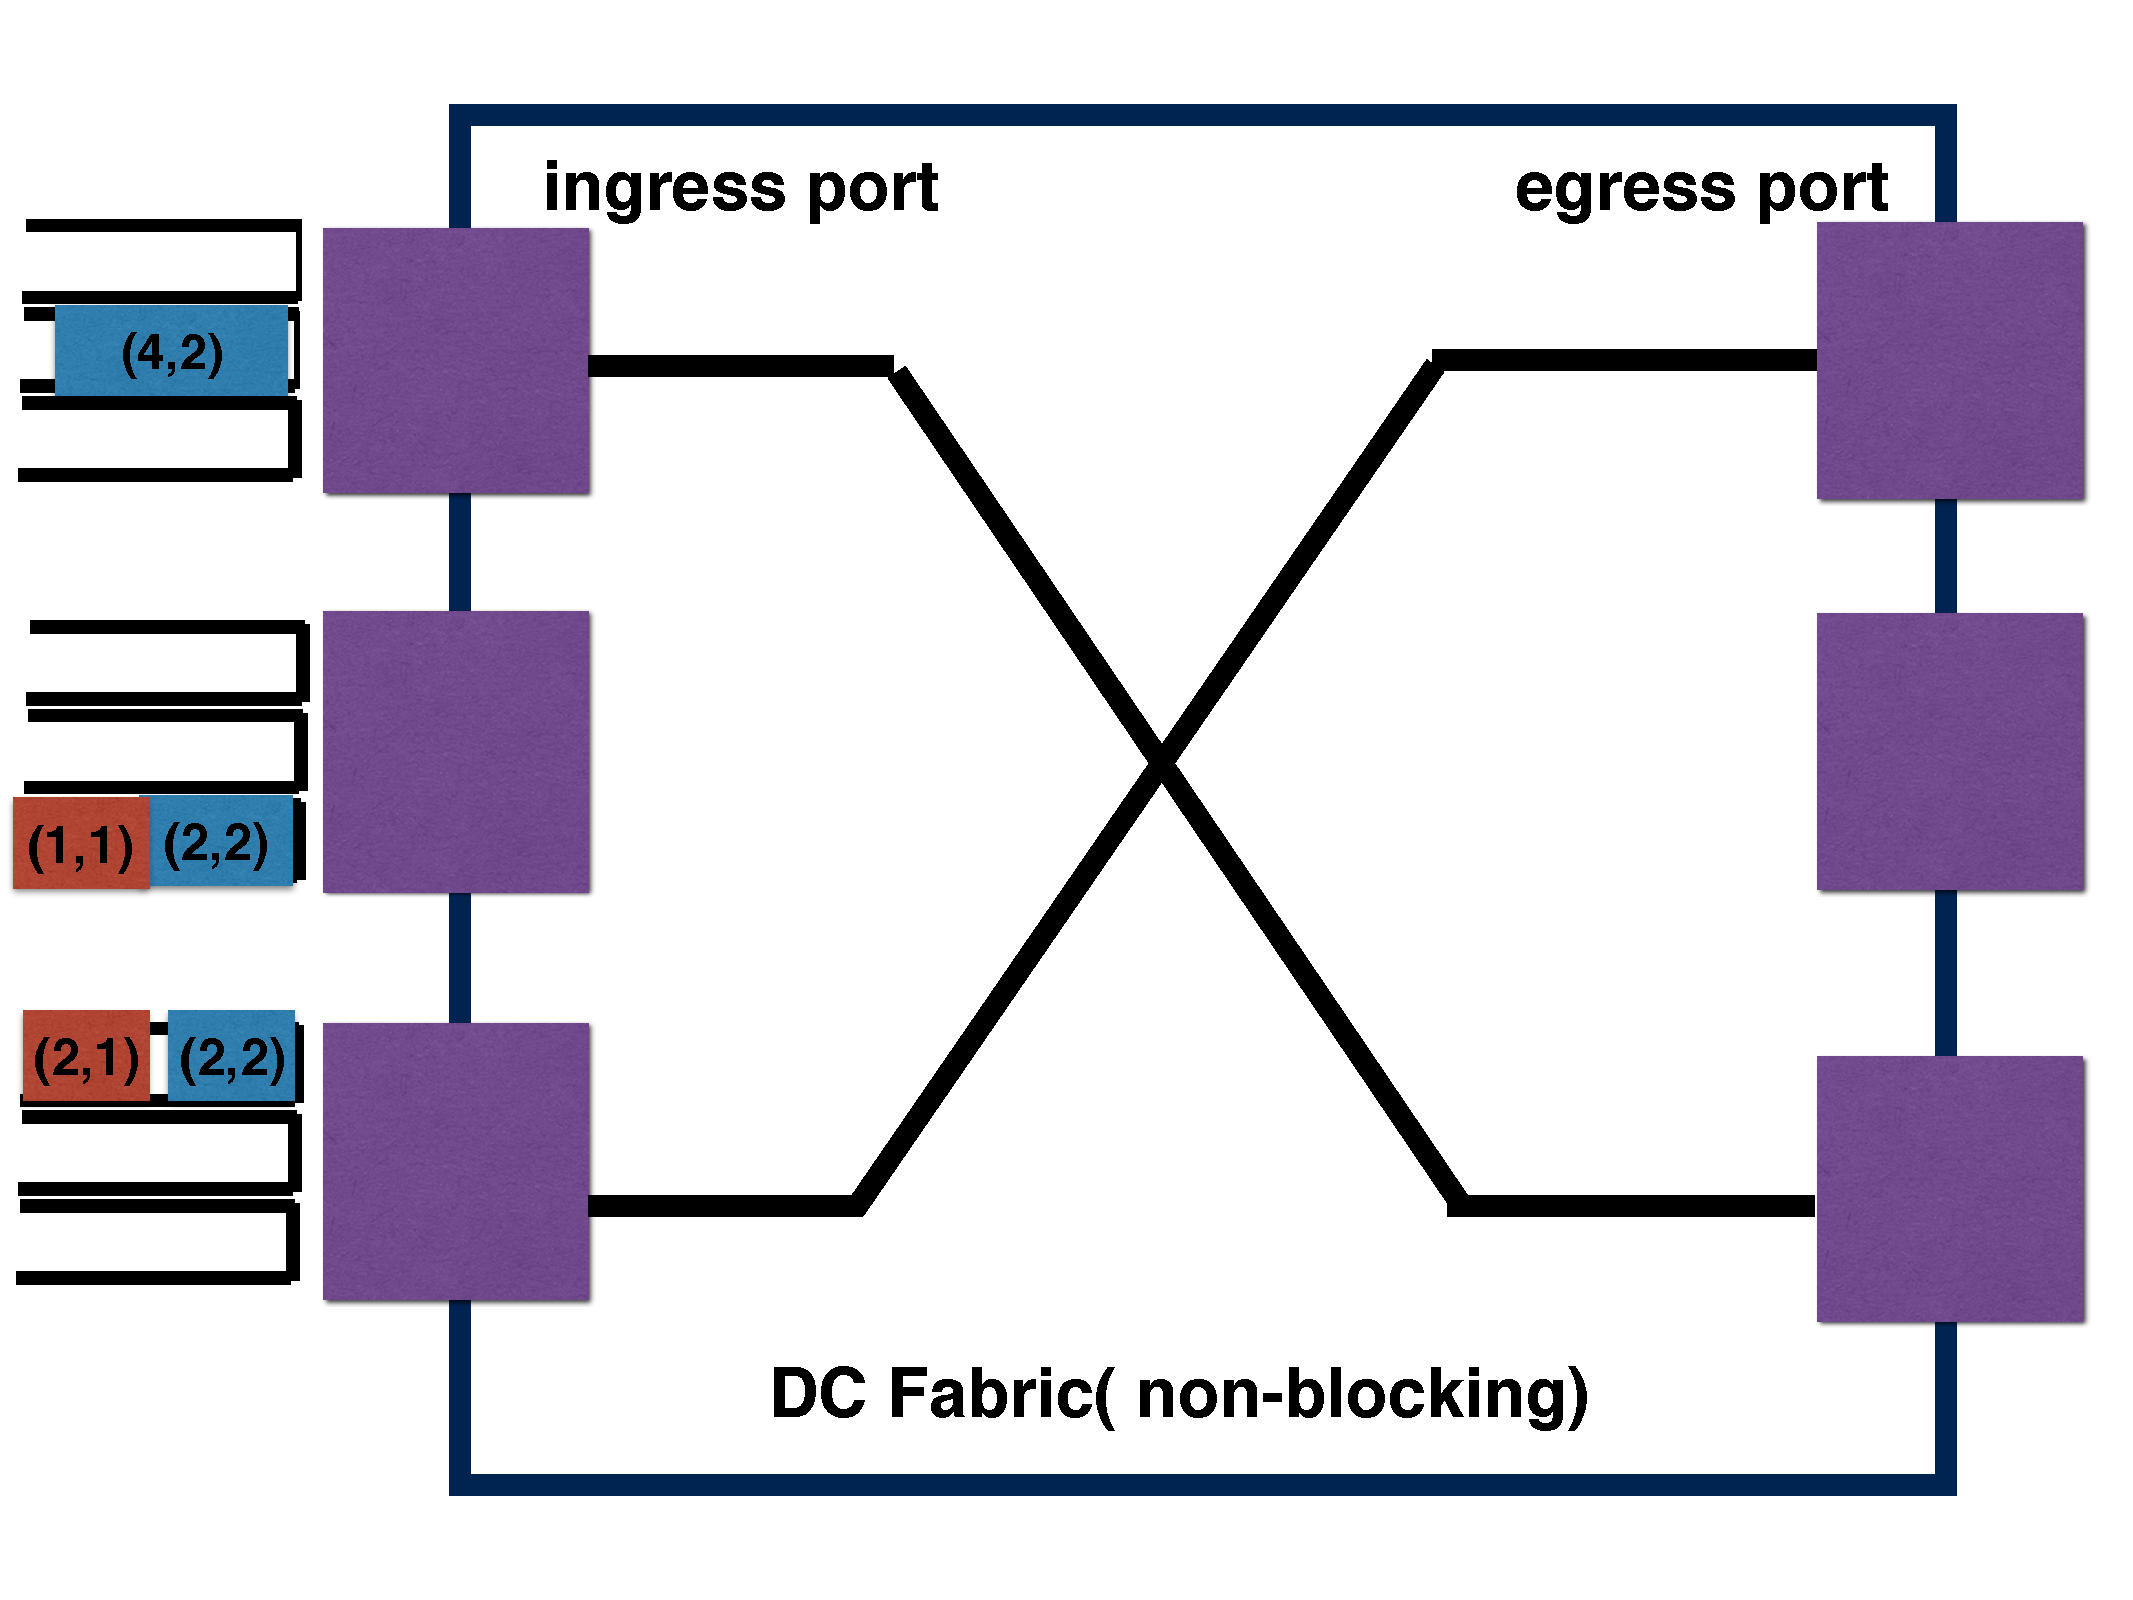
\includegraphics [width=0.8\columnwidth] {./figs/background/non_blcoking.pdf}
\caption{Data center as non-blocking fabric: in this fabric, congestion only occurs at the ingress ports or egress ports}
\label{Datacenter-nonblocking-fig}
\end{center}
\end{figure}



Recent researches have regardedc  the data center network as  a big giant non-blocking switch which interconnects all the machines. Just as Fig. \ref{Datacenter-nonblocking-fig} shows.
Under this assumption,  congestion only occurs at the egress and ingress ports. Flows always contend for the ingress and egress ports' network resources. It is practical because of recent advances in full bisection bandwidth topologies distribute flows efficiently. Also, some previous study\cite{chowdhury2015efficient}\cite{huang2016sunflow}\cite{chowdhury2014efficient}\cite{pFabric} use this 
model to design the algorithms. To simplify the problem, in this paper,  we follow the assumption and only compute the ingress and egress ports' congestion. 

\subsection{Application importance semantics}

Applications in data center share the networks resources. Different applications have different level of importance. The more emergency applications hope to 
get more bandwidth. Some previous study\cite{D2TCP}\cite{D3}\cite{zhang2015more} uses deadline to present the emergency of applications. Deadline indeed emphasizes 
a minimal bandwidth constraints on applications. In reality, in data center network, applications do not need a real lower bound of bandwidth, they are urgent and just want
to transfer as quickly as possible. To present the level of emergency, we incorporate weight to present the urgent level of applications. Applications whose level of emergency is high, will 
have a larger weight. Instead of trying to minimize coflow completion time, we try to minimize coflow weight completion time. 


%\begin{table}[th!]\label{model_define}
%\begin{center}
%\tabcolsep=0.11cm
%\begin{tabular}{cc}
%\hline\hline \\[-0.7ex]
%{\bf Symbol} & {\bf Meaning} \\ 
%$N$& Number of servers, indexed by $i=1,\ldots,N$ \\
%$\psi$ & coflow, each coflow $\psi $ contains many flows\\
%$f_{\psi}^{j}$ & coflow $\psi$'s jth subflow \\
%$\Psi$ & coflow set, elements in this set are $\psi_1$,$\psi_2$,$\psi_3$..\\
%$C_{\psi}^{j}$ & the completion time of $f_{\psi}^{j}$ \\
%$C_{\psi}$ & the completion time of $\psi$ \\
%$P_{\psi}^{j_{in}}$ & ingress port for $f_{\psi}^{j}$\\
%$P_{\psi}^{j_{out}}$ & egress port for $f_{\psi}^{j}$\\
%$L_{\psi}$ & number of  flows in coflow  $\psi$ , indexed by   $i=1,\ldots,N$\\
%$R_{P} $ &\ remaining capacity for port P that is measured by the system\\
%
%$w_{\psi}$ & weight for task $\psi$ \\
%$p_{\psi}^j$ & transfer time for flow  $f_{\psi}^{j}$ \\
%$d_{\psi}^j$ & volume for flow  $f_{\psi}^{j}$ \\
%$r_{\psi}^{j}$ & start (release) time of flow  $f_{\psi}^{j}$ \\
%
%\hline\hline \\[0.5ex]
%\end{tabular} \caption{Main notation.}
%\end{center}
%%\vspace{-0.3in}
%\end{table}
%\vspace{-.1in}


\subsection{Problem formulation}

In this subsection, we consider the offline schedule problem of minimizing weight coflow completion problem. There are m machines connecting to the data center fabric, thus according to the non-blocking model fabric as Fig. \ref{Datacenter-nonblocking-fig} shown, there are m ingress ports and m egress ports. Assume there are n coflows to be scheduled. Each coflow involve $m \times m $ parallel flows. The k-th coflow is a collection flows denoted by $F^{(k)}=\{f^k_{i,j}|1 \leq i\leq m,1\leq j \leq m\}$, where $f^k_{i,j}$ is the flow size sends from host i to host j. In reality, there are no flows sending from host i to host j. Under this condition $f^k_{i,j}=0$.

Let $C_{i}$ denote the completion time coflow $F_{i}$. Weight of coflow $F_{i}$ is $w_i$The capacity of each ingress and egress ports is 1. Just as \cite{chowdhury2014efficient}, we now define the Weight Coflow Completion Optimization (WCCO) problem as follows:

\begin{eqnarray}
& \d {\rm minimize} & \sum_{i=1}^{n} w_{i} C_{i} \label{eq:WCCO-SC} \\
& \d{\rm s.t.} & \sum_{\forall l:C_l<C_k}\sum_{i=1}^{m}f_{i,j}^{(l)} \leq C_k  \label{eq:ingress_constraint} \\
&& \sum_{\forall l:C_l<C_k}\sum_{j=1}^{m}f_{i,j}^{(l)} \leq C_k   \label{eq:egress_constraint}
\end{eqnarray}

(\ref{eq:WCCO-SC}) is the optimize goal. The goal is to try to minimize weight completion time. (\ref{eq:ingress_constraint}) and (\ref{eq:egress_constraint}) are ingress and egress ports bandwidth capacity constraints.

\subsection{NP-hard and problem equivalent proof} \label{np-hard-proof}

%.  Assume there are N machines (indexed by 1,2,...N) connecting to the data center network. Each machine connects to the giant switch through the link with the capacity of R. We define the coflow set as $\Psi$ and each coflow contains many flows($f_{\psi}^{j}$) whose source ($P_{\psi}^{j_{in}}$ )and destination($P_{\psi}^{j_{out}}$ ) are known beforehand. The weight for coflow $\psi$ is $w_{\psi}$.
%$p_{\psi}^j$  is transfer time for flow  $f_{\psi}^{j}$, $r_{\psi}^{j}$ is the start (release) time of flow  $f_{\psi}^{j}$ and $d_{\psi}^j$ is volume for flow  $f_{\psi}^{j}$ .  Details for our model is shown at Table \ref{model_define}.

We give the definition of Concurrent Open Shop problem, then we prove WCCO is equivalent.  The problem of concurrent open shop problem can be described as: considering that a job consists of up to m different components to be processed on a specific one of m dedicated machines. Components are independent of each other, such that components of the same job can be processed in parallel on different machines. A job is completed once all of its components are completed \cite{roemer2006note}. The goal of concurrent open shop problem is to try to find a 
sequence to minimize weight completion time or to find a sequence to let more jobs finish before deadline\cite{chen2000supply}.

\begin{proposition} \label{WCCO-eq}
Minimizing weight completion time of coflows is equivalent to minimizing weight  completion time of jobs in concurrent open shop problem.
\end{proposition}

To prove proposition \ref{WCCO-eq}, Firstly we consider the single coflow condition. Let $L(F^{(k)})$ denote the maximum load that the coflow $F^{(k)}$ exerts. The definition of  $L(F^{(k)})$ is as follows:
\begin{eqnarray} \label{load_define}
L(F^{(k)})=max \{max_{i}\sum_{j=1}^m f_{i,j}^{(k)},max_{j}\sum_{i=1}^m f_{i,j}^{(k)}\}
\end{eqnarray}

(\ref{load_define}) gets the larger loads of ingress port and egress port. For the single coflow situation, weight completion time of coflow $L(F^{(k)})$ can be computed as $w_k*L(F^{(k)})$.

Secondly,  assume there are two coflows $F^{(k)}$ and $F^{(l)}$, The priority of coflows indicates the schedule sequence of them.
Let  P(.) denote the priority of coflow and the schedule sequence of  $F^{(k)}$ and $F^{(l)}$ can be defined as  definition \ref{sequence_definition}.

\begin{definition} \label{sequence_definition}
 For any two coflows  $F^{(k)}$ and $F^{(l)}$, $P(F^{(k)}) \prec P(F^{(l)})$ means coflow  $P(F^{(k)})$ has lower priority value than $P(F^{(l)})$ and scheduler should schedule $F^{(k)}$ before $F^{(l)}$. $P(F^{(k)}) \succ P(F^{(l)})$ means coflow  $P(F^{(k)})$ has higher priority value than $P(F^{(l)})$ and scheduler should schedule $F^{(k)}$ after $F^{(l)}$.
\end{definition}

For two coflows, we can define the operation adding of them as follows:
\begin{definition} \label{add_definition}
 For any two coflows  $F^{(k)}$ and $F^{(l)}$. We can define the single new  $m \times m $ coflow $F^{(n)}= F^{(k)} \bigcup F^{(l)}$, whose flow demand $f^n_{i,j}=f^k_{i,j}+f^l_{i,j}$.
 \end{definition}
 
 
 \begin{lemma} \label{two-coflow}
For the two coflows, say $F^{(k)}$ and $F^{(l)}$, the optimum of $\mathbb{\min \max} \{C_l,C_k\}$ is $L( F^{(k)} \bigcup F^{(l)})$
\end{lemma}
\begin{IEEEproof}
Firstly, For the single coflow n, its optimal completion time $L(F^{(n)})$ . Then we prove that $L( F^{(k)} \bigcup F^{(l)})$ is the low bound of
$\mathbb{\min \max} \{C_l,C_k\}$. It is obvious that   $\mathbb{\max}\{C_l,C_k\} \ge L( F^{(k)} \bigcup F^{(l)})$. This is because if $\mathbb{\max}\{C_l,C_k\} < L( F^{(k)} \bigcup F^{(l)})$, then
both $F^{(k)}$ and $F^{(l)}$ can finish before $L( F^{(k)} \bigcup F^{(l)})$. According to Definition \ref{add_definition}, $L( F^{(k)} \bigcup F^{(l)})=L(F^{(n)})$, so coflow  $F^{(n)}$ can finish before 
$L( F^{(n)})$. This is contradict to the optimal completion time of $F^{(n)}$ is $L(F^{(n)})$.
\end{IEEEproof}

Lemma \ref{two-coflow} indicates that for two coflow system, $F^{(k)}$ and $F^{(l)}$, the optimal schedule completion time of the latter one is $L( F^{(k)} \bigcup F^{(l)})$. Then for weight completion time $\min\{w_l*C_l+w_k*C_k\}$, if $P(F^{(k)}) \prec P(F^{(l)})$, the optimal value of $\min\{w_l*C_l+w_k*C_k\}$ is $w_k*L(F^{(k)})+w_l*L( F^{(k)} \bigcup F^{(l)})$. Else if $P(F^{(k)}) \succ P(F^{(l)})$, the optimal value of $\min\{w_l*C_l+w_k*C_k\}$ is $w_l*L(F^{(l)})+w_k*L( F^{(k)} \bigcup F^{(l)})$.

Thirdly, we generate this conclusion to coflow set. Assume there are g coflows.  Let $\gamma(k)$ denote the priority sequence of coflow k.  $WT(\gamma)$ denote the weight completion time under priority permutation $\gamma$:

\begin{eqnarray} \label{weight_completion_gamma}
WT(\gamma)= \sum_{i=1}^gw_i*L(\sum_{j=1}^i F^{(\gamma|j)})
\end{eqnarray}

So, Minimizing the weight coflow completion  for a given set of coflows is equivalent to finding a permutation  $\gamma$ for them (i.e., optimal priority permutation), so that WT is minimized. so far, we have changed the problem of minimizing coflow weight completion time has been changed to finding the optimal order permutation for them, which is quite similar to concurrent open shop problem. They are equivalent indeed. Next, we will describe the equivalence of them. 

For each coflow $F^{(k)}$, let $f_i^{k}=\sum_{j=1}^mf_{i,j}^{k}$, for ingress ports i=1,2...m and  $f_{j+m}^{k}=\sum_{i=1}^mf_{i,j}^{k}$ for egress ports j=1,2...,m. Substitute $f_i^{k}$ and $f_{j+m}^{k}$ into (\ref{weight_completion_gamma}), then we get the fact that find the permutation of coflow is the same case as finding the optimal sequence for minimizing weight job completion time in concurrent open shop problem. In the problem, there are 2m jobs donated as $f_i^{k}$ and $f_{j+m}^{k}$ to be performed on 2m machines.  The machine index is denoted as i=1,2,..2m. On the contrary, by letting flows deriving from the same ingress port drain by the same egress port, we can construct concurrent open shop problem's corresponding coflow schedule problem.

Now, we have proved proposition \ref{WCCO-eq} which is the equivalence of minimizing coflow weight completion time and minimizing job weight completion in concurrent open shop problem.
According to \cite{roemer2006note} and \cite{mastrolilli2010minimizing}, finding a sequence of minimizing weight job completion time is NP-hard. As the problem is equivalent to minimizing coflow weight completion time, so finding a permutation of coflow to minimize weight coflow completion time is also NP-hard.

\section{Algorithm design and analysis}\label{algorithm}
 
Learning from the conclusion of \ref{np-hard-proof}, we can learn that minimizing coflow weight completion time is indeed to find a permutation of   $\gamma$ that make the value of WC minimize. As
the hardness of the problem is NP-hard \cite{roemer2006note}, so efficient heuristic is needed. In this section, we first introduce a 2-approximate algorithm, then we conclude the idea of the algorithm and proposal an online algorithm for coflow weight completion optimization problem. At last we compare the online and offline version of the two algorithm.
 
 
\subsection{Weight coflow completion time offline algorithm}
Currently, the best known result for the problem is a permutation based greedy algorithm, which is proven to be 2-approximation\cite{kumar2011lp,mastrolilli2010minimizing}, and we can also find a 2-approximate algorithm for minimizing coflow weight completion time according to this. We first change the  2-approximate algorithm from \cite{mastrolilli2010minimizing} which intends to minimize weight job completion time to minimize coflow weight completion time. 
 
 \begin{algorithm} \label{offline}
 \caption{2-approximation offline algorithm}
 \begin{algorithmic}[1]
 \renewcommand{\algorithmicrequire}{\textbf{Input: }}
 \renewcommand{\algorithmicensure}{\textbf{Output:}}
 \REQUIRE n,m,$f_{i,j}$
 \ENSURE  $\gamma$
  \STATE $\gamma:\{1,2,...n\} \gets N$
  \\ \textit{$UC\gets\{1,2,3...n\}$}
  \\ \textit{$P\gets\{1,2,3...m\}$}
  \\ \textit{$W\{1,2,...n\}\gets\{w_1,w_2,w_3...w_n\}$}
  \STATE $L_i^{(k)}= \sum_{j=1}^mf_{i,j}^{(k)}$ for all k $\in$ N and i $\le$ m
   \STATE $L_{j+m}^{(k)}= \sum_{i=1}^mf_{i,j}^{(k)}$ for all k $\in$ N and j $\le$ m
    \STATE $L_i=\sum_{k \in N}L_i^k$ for all i $\in$ P
   \FOR{i $\in\{n,n-1,n-2...1\}$ }
  \STATE u=$\arg \max \limits_{k \in N}L_k$
   \STATE $\gamma[i]$=$\arg\min \limits_{F \in UC} W[F]/L_u^{(F)}$
   \STATE $\theta=W[\gamma[i]]/L_{u}^{\gamma[i]}$
   \STATE W[j]=W[j]-$\theta$*$L_u^{(j)}$ for all j $\in$ UC
   \STATE $L_j=L_j-L_j^{\gamma[i]}$ for all j $\in$  P
   \STATE $UC = UC \setminus\{\gamma[i]\}$
  \ENDFOR
 \end{algorithmic} 
 \end{algorithm}
 
 
 Algorithm 1 is the description of minimizing weight coflow completion time. 
 The algorithm 's elementary operations is O(n(m+n)), where n is the number of colfows to be scheduled and m is the number of machines in data center network.
 The input of the algorithm is m,n and  $f_{i,j}$, which indicates that there are n coflows to be scheduled and each coflow will have $d_{i,j}^k$ size of flows to transfer
 from machine i to machine j, the total number of machines is m. Output of the algorithm is $\gamma$, which indicates the scheduling permutation of coflows.
 
 Line1 does some initialism of the operation. UC is the set of coflows to be scheduled, W is the weight set of each coflow and P is the port set. Line2-Line4 computes the 
 load on each port. Load of each ports is the plus of flow size that goes through the port. Line5 - Line12 decides the schedule permutation sequence. Line6 finds the maximum 
 port which owns the heaviest load. Then Line7 finds the corresponding coflow which has the minimal ration of weight and load on that machine. Line8-Line10 is the adjust process.
 Line11 gets rid of this coflow from the unschedule sets. Algorithm 1 will generate $\gamma$ which is the permutation of coflow schedule sequence.
 
 Although the 2-approximate algorithm has been proved to work well \cite{mastrolilli2010minimizing}, it has some deficiencies that constraints its usage in practice:
 
 \begin{itemize}[\IEEEsetlabelwidth{Z}]
\item The algorithm is an offline version, it assumes that coflow arrives simultaneously, indeed, in data center network, coflows wiil arrive dynamically in practice\cite{chowdhury2012coflow,chowdhury2015efficient}. If we use the offline version algorithm, we have to recompute the schedule sequence of coflows and this will
emphasize heavy load on the controller if coflow arrive too frequency.
\item The 2-approximate greedy algorithm's elementary operations is O(n(m+n)). If the number of machines in datacenter or the number of coflows to be scheduled is too large. It will take 
a long time to get the results of $\gamma$.
\end{itemize}

 To make the algorithm work practically and efficiently in data center network, we have to make some relaxations.
 
%\begin{figure}
 %\vspace{-8mm}
  %  \begin{minipage}{.47 \textwidth}
   %  % \begin{algorithm}[5]
   %     \caption{Minimize coflow completion time offline algorithm}
%        \label{alg:coflow_offline}
%        %\begin{algorithmic}
        %\STATE \textbf{for } every port :
        %\STATE \hspace{\algorithmicindent}  \textbf{for } every task $\psi$:
       %  \STATE \hspace{\algorithmicindent} \hspace{\algorithmicindent} \textbf{for} f in  $\psi$:
    %      \STATE \hspace{\algorithmicindent} \hspace{\algorithmicindent}\hspace{\algorithmicindent}  \textbf{if} f goes through port P:
 %          \STATE \hspace{\algorithmicindent} \hspace{\algorithmicindent}\hspace{\algorithmicindent}\hspace{\algorithmicindent} load[port]+=p[$\psi$][f]
%\STATE k=n
%\STATE\textbf{while} $k>1:$
%\STATE\hspace{\algorithmicindent} u=$\max \limits_{i \in N}load[i]$
%\STATE Compute current objective value $B^{(0)}$
%\STATE \textbf{do}
%\STATE \hspace{\algorithmicindent} Solve Convex Problem { Prob\_Z} to get $z_{i,t}$ for given $\pi_{i,j,t}$ for all $i$
%\STATE \hspace{\algorithmicindent} Set $k_{L,i,t}=0$, $k_{U,i,t} = k_i$
%\STATE \hspace{\algorithmicindent}\textbf{do}
%\STATE \hspace{\algorithmicindent} \hspace{\algorithmicindent} Solve Convex Problem Prob\_$\Pi$ to get $\pi_{i,j,t}$ for given $z_{i,t}, \  k_{L,i,t}, \  k_{U,i,t}$ for all $i,j$
%\STATE \hspace{\algorithmicindent} \hspace{\algorithmicindent} Let $i_1 = \arg\max$ (fractional part of $\sum_{j=1}^m \pi_{i,j,t}$)
%\STATE \hspace{\algorithmicindent} \hspace{\algorithmicindent}$k_{L,i_1,t}= k_{U,i_1,t} = ceil(\sum_{j=1}^m \pi_{i,j,t})$
%\STATE \hspace{\algorithmicindent} \textbf{while} $\sum_i frac(\sum_{j=1}^m \pi_{i,j,t})>0$
%\STATE \hspace{\algorithmicindent}Compute new objective value $B^{(c+1)}$,  Update  $c=c+1$
%\STATE {\bf while} $B^{(c)}-B^{(c-1)}>\epsilon$
        %\end{algorithmic}
      %\end{algorithm}
    %\end{minipage}
   % \vspace{-.25in}�
 % \end{figure}
  
  
 

%The main process of Yosemite is as follows: There are two main process on the sender
%the sending process and the 
%When a coflow arrives, the corresponding sender will
%send the information to the master. Senders send flow information to maters.
%every T time, all senders send corresponding flow information to the master.
%The master will collect the information of all coflows and use the online algorithm to compute the sequence of the coflow.
%Then the master will send the sequence to the senders. The senders use the sequence to decide the bandwidth of each flow and 
%send flows with the result of the computation.
%
%We combine centralized with distributed scheduling method in our system.  The master is the brain of our method, it summarizes the
%information from the endpoints. Each machine in data center has a slaver damon. The slaver generates coflow information and sends 
%the flow information to master. After the sequence computation, it then use its rate limiter to do rate control.
%
%Priority queue is used at the sender side to help do the scheduling problem. Just as Fig .\ref{queue-fig}  shown.  There are N queues at the sender side,
%each queue has a priority $w_j$.  The number of flows that queue j can accommodate is $E_j$. Note, the lowest queue can accommodate infinite number of
%flow in reality.   

%\begin{figure}[b]
%\begin{center}
%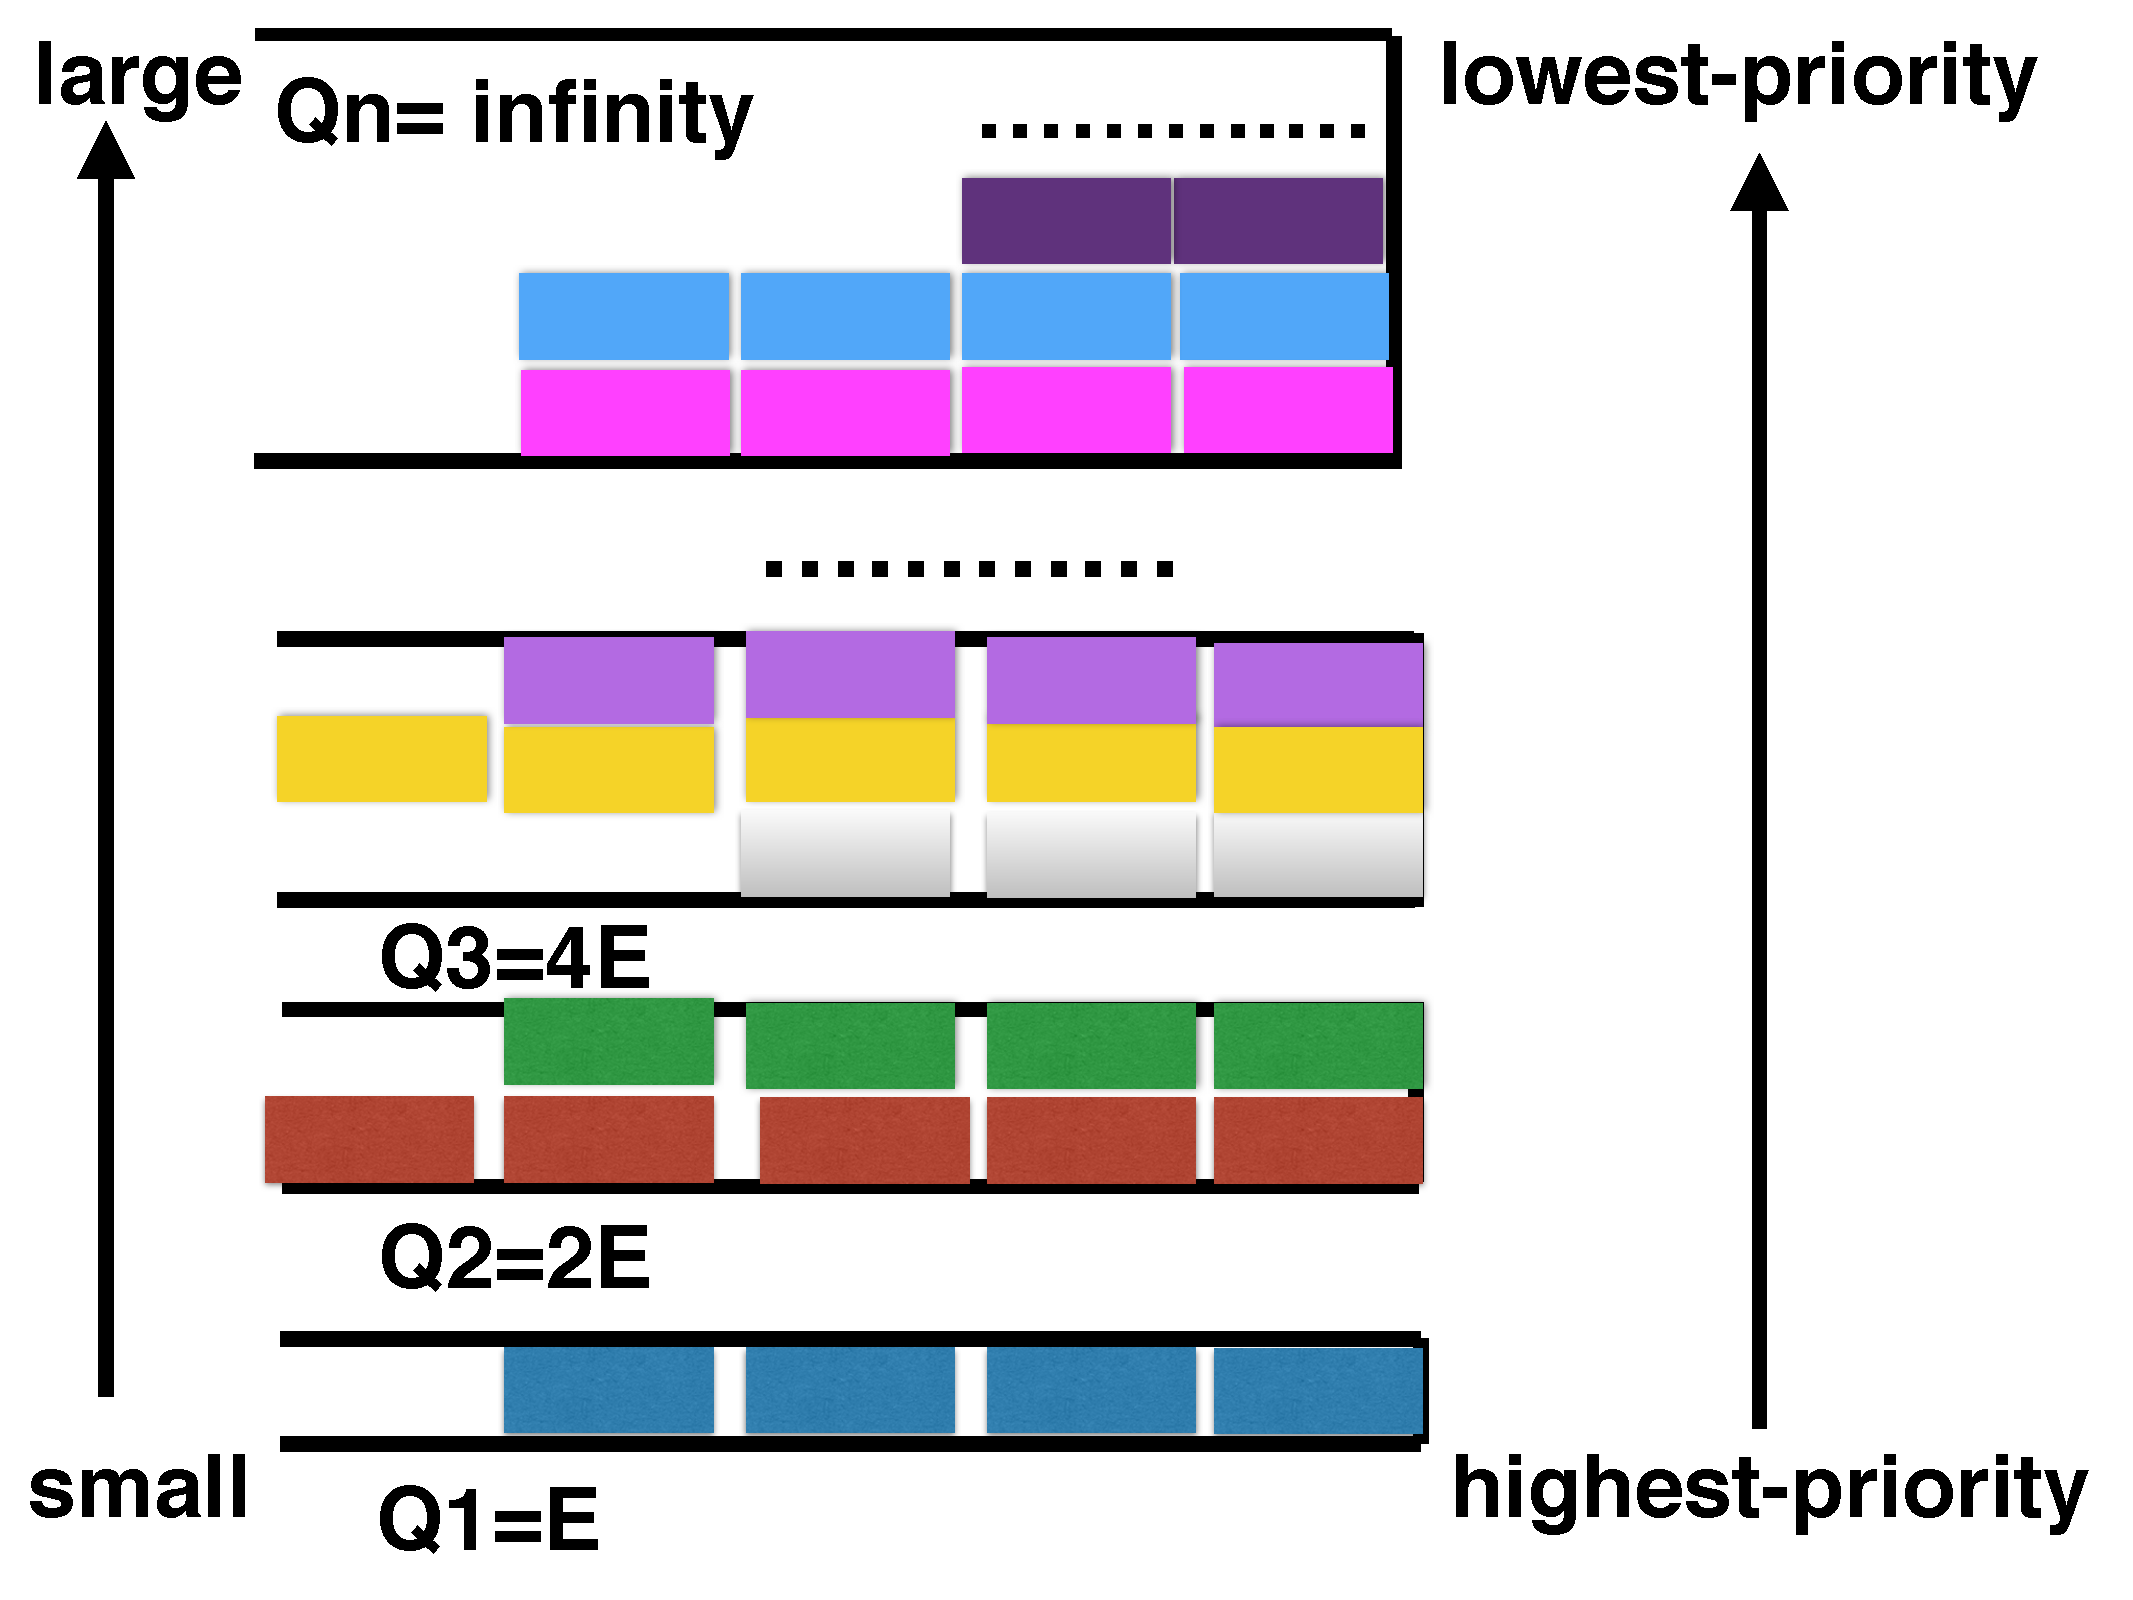
\includegraphics [width=0.8\columnwidth] {./figs/system/queue.pdf}
%\caption{Weight Priority Queue: from the bottom, the size of queue become larger and the priority lower }
%\label{queue-fig}
%\end{center}
%\end{figure}

%
%As the sequence of coflows is updated every T, however, in practice, some flows are always short and wait for T time may lead to bad performance.
%As a result, in our system, we set a threshold K,  flows whose size is smaller than K will get the lowest priority and this can avoid the condition of starvation.


\subsection{From offline to online}

The 2-approximate algorithm decides the schedule position for coflow by the ratio of weight and load on that machine. In reality, today's datacenters generally assign jobs with load balancing \cite{dean2008mapreduce}, as a result, the schedule process does not need to take the load diversity of ports into account. When a new coflow comes,  we can set the lowest priority to the coflow which has maximum per-port load. Then we get the online approach of coflow weight completion schedule.

\begin{algorithm} \label{online}
 \caption{Online approach to minimize weight completion time}
 \begin{algorithmic}[1]
 \renewcommand{\algorithmicrequire}{\textbf{Input: }}
 \renewcommand{\algorithmicensure}{\textbf{Output:}}
 \REQUIRE Coflow set $\mathcal{C}$ ; number of hosts m; remaining flow demands $d_{i,j}$ from port i to port j, where $1 \leqslant i
 \leqslant m$,$1 \leqslant j \leqslant m$
 \ENSURE  $\gamma$
  \STATE $W\{1,2,...n\}\gets\{w_1,w_2,w_3...w_n\}$
  \STATE $L_i^{(k)}= \sum_{j=1}^mf_{i,j}^{(k)}$ for all k $\in$ $\mathcal{C}$ and i $\le$ m
   \STATE $L_{j+m}^{(k)}= \sum_{i=1}^mf_{i,j}^{(k)}$ for all k $\in$ $\mathcal{C}$and j $\le$ m
    \STATE  $g^{(k)}$=$ \max \limits_{1 \le i \le 2m}L_i^{(k)}$ for all k $\in$$\mathcal{C}$ 
     \STATE  $\alpha^{(k)}$=W[k]/$g^{(k)}$ for all k $\in$ $\mathcal{C}$ 
     \STATE sort[$\alpha^{(1)}$,$\alpha^{(2)}$,$\alpha^{(3)}$...$\alpha^{(n)}$] in non-decreasing order and set the result to $\gamma$
     \end{algorithmic} 
 \end{algorithm}

Algorithm 2 is the online version of the 2-approximate. Different from the 2-approximate offline algorithm,  the online algorithm makes the relaxation that ignoring the load difference of
each port. Line2-Line4 computes the load of every coflow. Similar to \cite{chowdhury2014efficient}, the load of each coflow is:

\begin{eqnarray} \label{weight_completion_gamma}
g^{(k)}=\max(\max \limits_i \frac{ \sum_{j=1}^mf_{i,j}^{(k)}}{Rem(P_i^{(in)})},\max \limits_j \frac{ \sum_{i=1}^mf_{i,j}^{(k)}}{Rem(P_j^{(out)})})
\end{eqnarray}

$Rem(P_i^{(in)})$ denotes the remaining port capacity of ingress port $P_i^{(in)}$. $Rem(P_j^{(out)})$ denotes the remaining port capacity of egress port $P_j^{(out)}$. 
In our assumption, the capacity of each port is 1. After computing the load of each coflow. We compute the ratio of weight and load at Line5.
At last, we sort the ratio of each coflow  in non-decreasing order. Comparing with Algorithm 1, instead of having the O(n(m+n)) for-do loop, Algorithm 2 only has the sort operation. Algorithm 2 is
called when a new coflow starts. If we use insertion sorting method, the elementary operations is O(logn), where n is the number of coflow to be scheduled. 

\subsection{Distance between the online and offline algorithm}

The online algorithm makes relaxation, so the scheduling algorithm becomes much easier. However, one may argue, how  is the performance of the online algorithm comparing with the 2-approximate algorithm. To compare the performance of the two algorithms, we use the trace of real traffic from facebook \cite{chowdhury2014efficient}. For the weight of coflows, we random set
a integer from 1 to 5.  Using our simulator \cite{YosemiteSim} that improves from Varys \cite{chowdhury2014efficient}, Fig. \ref{online-offline-fig} shows the result. 

We can see from Fig. \ref{online-offline-fig} that for 80\% of coflows, performance of the two algorithm has little difference. This means  comparing with the 2-approximate offline algorithm, the online-algorithm has  little performance loss($<20\%$). It is practical to use the online-algorithm in reality. More details comparison between the two algorithms are shown at Table \ref{tab:comparison}
% Sched-Mode   
\begin{table}[!htb]
          \centering
          \footnotesize
          \caption{Comparison between the two algorithms} \label{tab:comparison}
          \begin{tabulary}{\textwidth}{ccccr}
              \toprule
              \#Scheme  & \multicolumn{1}{c}{Sched-Mode} & Procedure & Performance \\
              \midrule
              \multicolumn{1}{r}{2-appr} & offline    & Complex     & High \\
              \multicolumn{1}{r}{Yosemite} & online    & simple     & High \\
              \bottomrule
          \end{tabulary}
      \end{table}

We conclude the online algorithm has little performance loss with simple procedure and online mode, so in our system we will introduce below, we prefer to use 
the online algorithm instead of the 2-approximate offline algorithm.


\begin{figure}[b]
\begin{center}
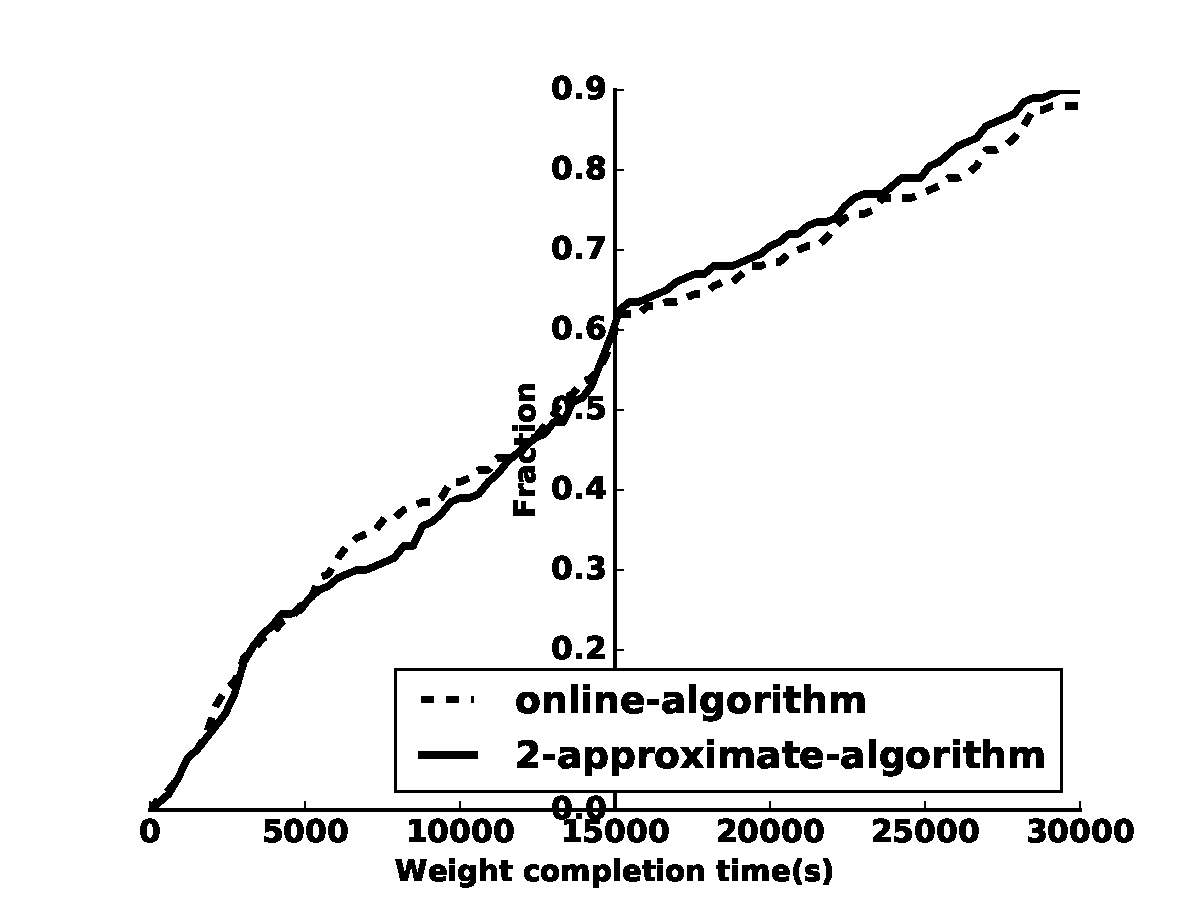
\includegraphics [width=0.8\columnwidth] {./figs/performance/online_offline.pdf}
\caption{performance comparison between 2-approximate algorithm and online algorithm}
\label{online-offline-fig}
\end{center}
\end{figure}


\section{Yosemite System}\label{Yosemite system}

In this section, we introduce the design of practical schedule system-Yosemite. We have evaluated Yosemite with about 4000 lines of java and scala, we learn some codes from Varys \cite{varys} and hadoop \cite{hadoop}. The code of Yosemite can be downloaded at \cite{Yosemite}. Similar to Varys \cite{varys}, we also use Akka \cite{Akka} for message transferring and kryo \cite{kryo} for object serialization. In this section, we first introduce the actors of Yosemite and the messages transferring between the actors. Then we introduce the API of Yosemite.
  \begin{figure}[b]
\begin{center}
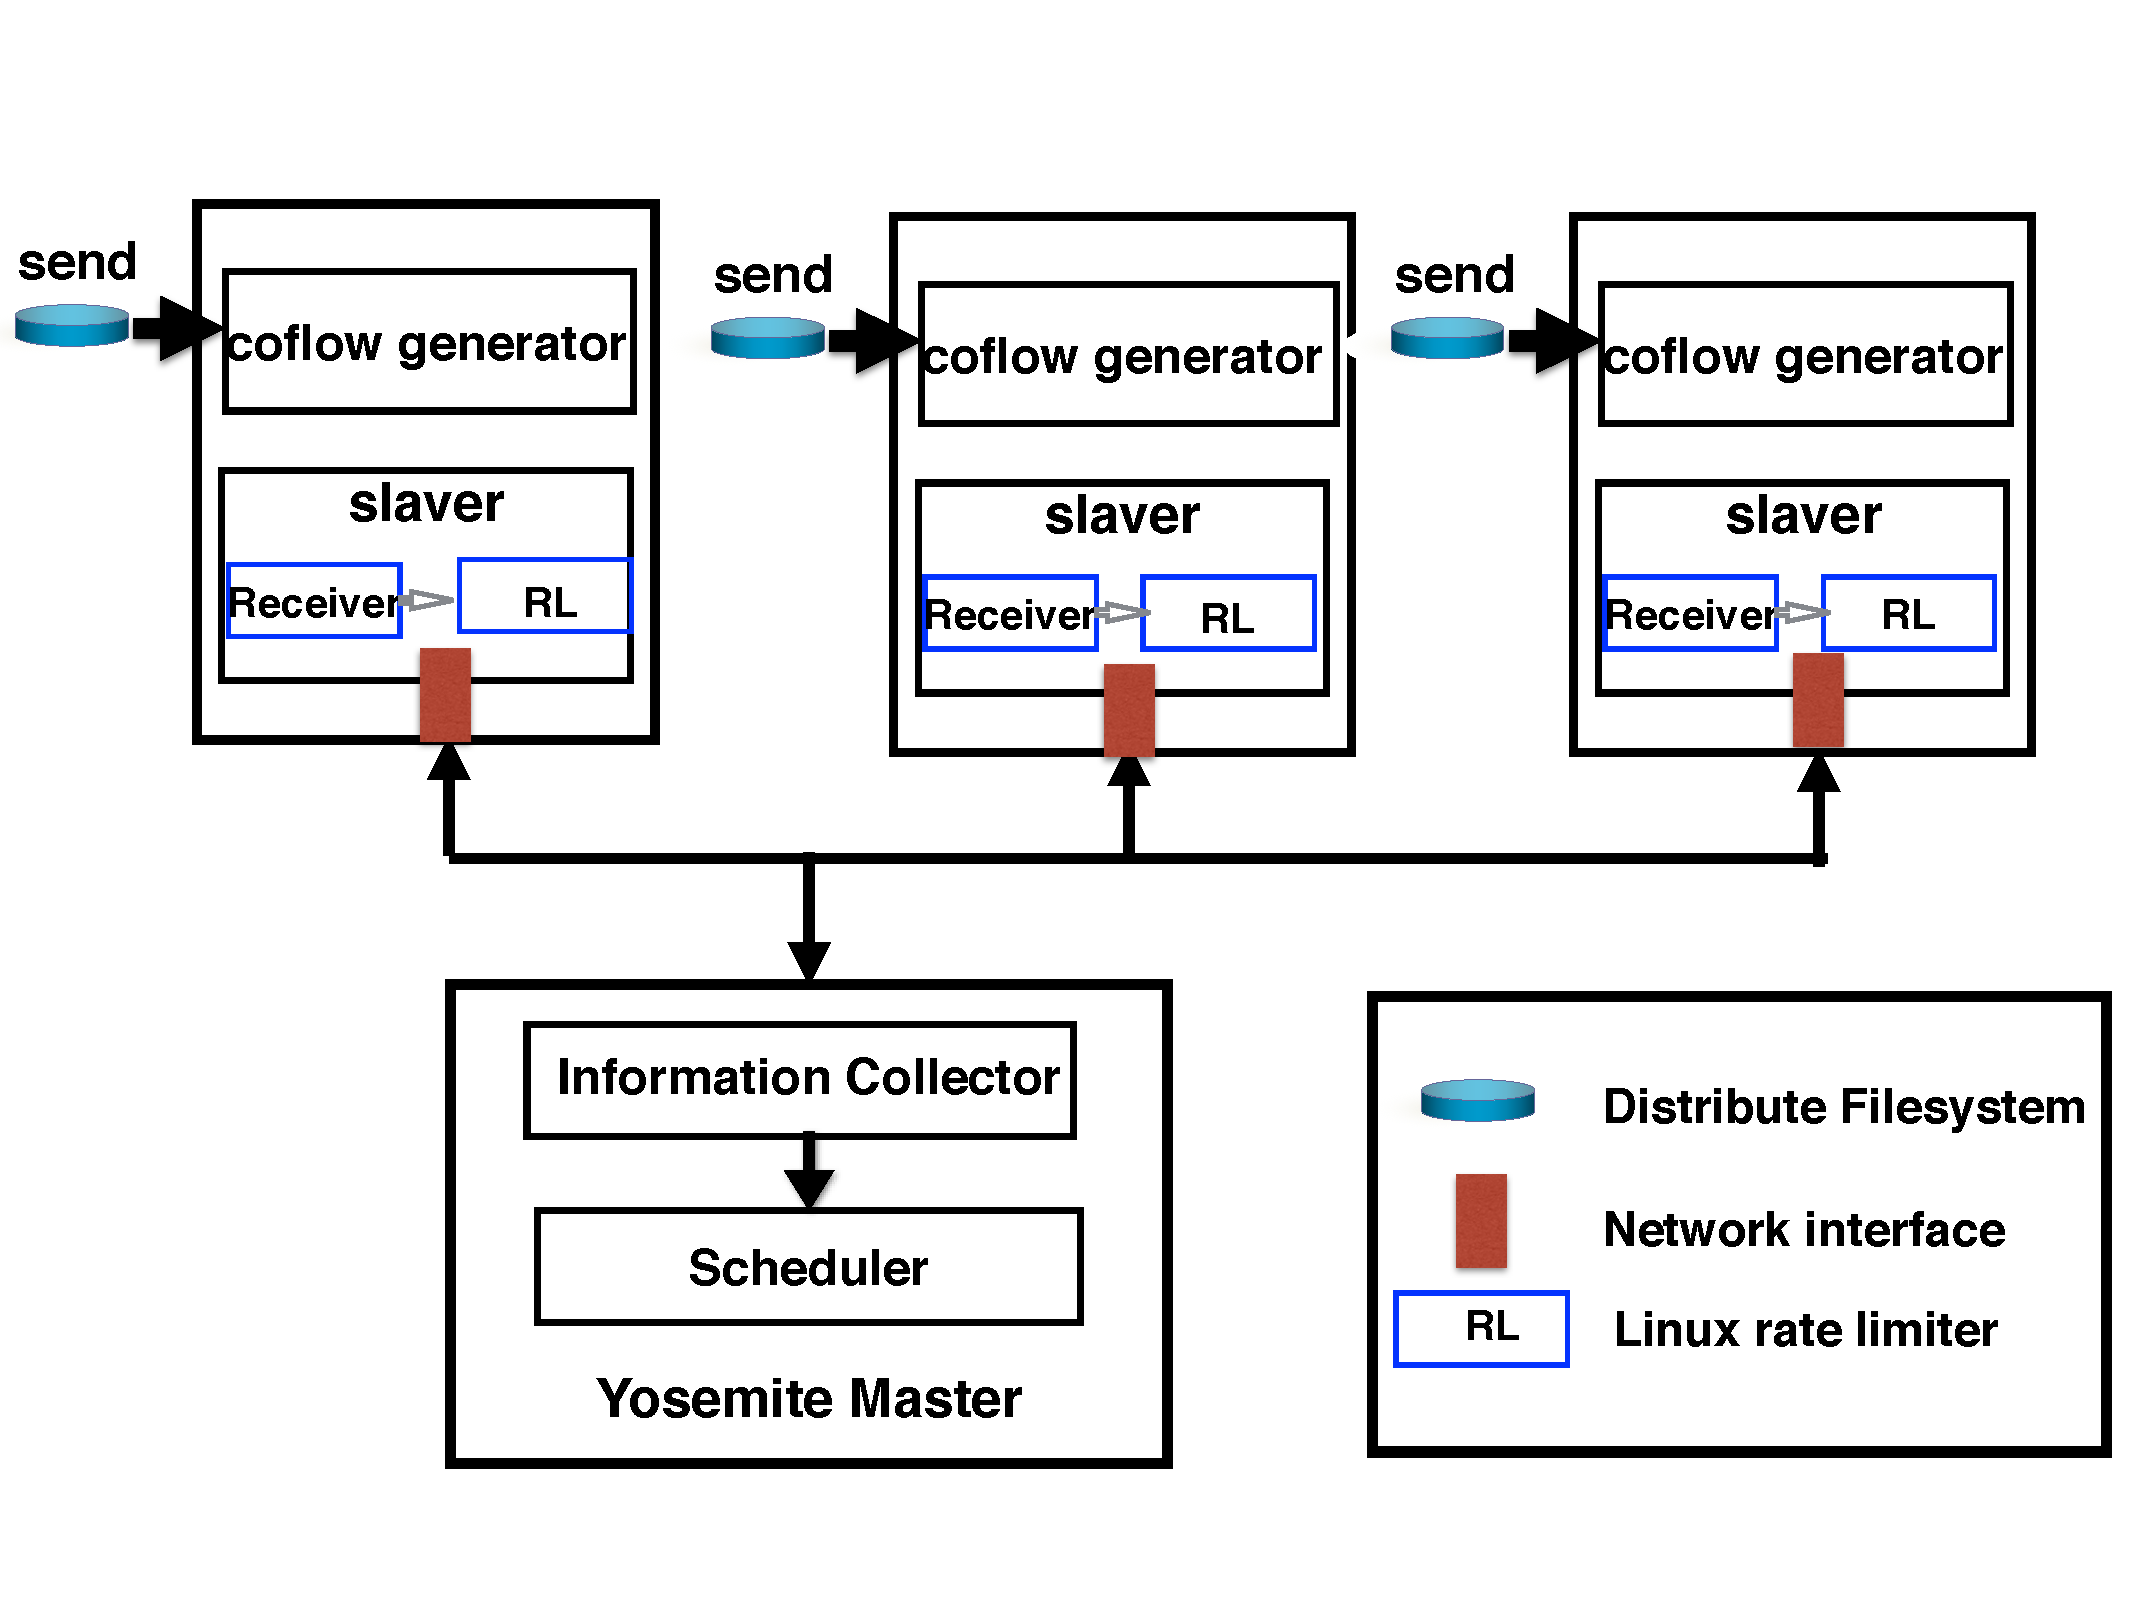
\includegraphics [width=0.8\columnwidth] {./figs/background/system.pdf}
\caption{Yosemite architecture. Computation frameworks interact with Yosemite through a client library}
\label{System-design-fig}
\end{center}
\end{figure}

\subsection{Actors and message transferring}  
\begin{algorithm} \label{bandwidth_allocate}
\caption{Procedure of bandwidth allocate}
\begin{algorithmic}[1]
\renewcommand{\algorithmicrequire}{\textbf{Input: }}
\renewcommand{\algorithmicensure}{\textbf{Output:}}
\REQUIRE Sorted coflow set $\gamma$, Remaining capacity for ports set $Rem(.)$
\ENSURE  bandwidth of each coflow, Remaing capacity for ports set $Rem(.)$
\FOR{k $\in \gamma$ }
 \STATE Compute Load $g^{(k)}$ according to (\ref{weight_completion_gamma})
 \FOR{$f_{i,j}$$ \in k$ }
 \STATE $b_{i,j}=f_{i,j}/g^{(k)}$
\STATE $Rem(P_i^{(in)})-=b_{i,j}$
\STATE $Rem(P_j^{(out)})-=b_{i,j}$
 \ENDFOR
\ENDFOR
\end{algorithmic} 
\end{algorithm}


\begin{algorithm} \label{procedure_master}
\caption{Procedure of the master}
\begin{algorithmic}[1]
\renewcommand{\algorithmicrequire}{\textbf{Input: }}
\renewcommand{\algorithmicensure}{\textbf{Output:}}
\REQUIRE Coflow F
\ENSURE  bandwidth of each flow 
\STATE $\mathcal{C}=\mathcal{C}\cup F $
\STATE Sort $\mathcal{C}$ according to Algorithm 2
\STATE Allocate bandwidth to $\mathcal{C}$ according to Algorithm 3
\STATE Distribute unused bandwidth to $\mathcal{C}$ for all ports
\STATE Send $b_{i,j}$ to corresponding Slaver
\end{algorithmic} 
\end{algorithm}
Just as Fig .\ref{System-design-fig} shows. Yosemite has two key actors: master and slaver. Master is the brain of the system. 
It collects coflow information from slaves, then computes the bandwidth of each coflow and  sends the result to slavers at last.  
Operations detail is shown as algorithm 4. This algorithm is called when a new coflow F arrives. Line1-Line2 tries to find the corresponding 
position for the coflow. The master uses the online algorithm 2 that tries to minimize weight coflow completion time. Line3 calls algorithm 3 which 
tries to allocate bandwidth to coflow according to the sequence that is computed at Line2. Algorithm 3 has two key steps. Line2 computes  load of
the coflow according to (\ref{weight_completion_gamma}). After compute the load of coflow, it then computes the bandwidth of coflow.  We regard the 
bottleneck flow bandwidth as the coflow bandwidth. All the flow that belongs to the coflow use the same bandwidth just as Line4 shown. After computing the 
bandwidth of flow, the master updates the port available bandwidth which as computing as Line5-Line6 shown in algorithm 3.  After computing the bandwidth of
each flow, the master send the result to slaver. Slavers throttle bandwidth to the value that computed by the master.

In reality, one of most diffcult things in writing correct distributed, concurrent, fault-tolerant and scalable applications is the communication between the components. 
Because messages transferring between components needs timely responds, keeping responsive in the face of failure, staying responsive under varying workload. In Yosemite,
we build our communication system based on Akka \cite{Akka}. With the help of Akka, Yosemite has high performance and fault-tolerance communication system.

\subsection{Work-conserving allocation}
Just using algorithm 3 to allocate bandwidth to each flows may lead to ports resource idle. To prevent this happening, we allocate the remaining bandwidth fair to the flows that 
sends from the ports just as Line4 shown at algorithm 4. With work-conserving allocation, resources can used more efficiency, so that less resources will be wasted.

\subsection{Fault-tolerance}
In Yosemite, master plays the role of brain of the system. It collects information from slaver and computes the bandwidth of each flows and sends the result to the slaver. In reality, the master
may be crushed. If this happened, the system can not work any more. To prevent this happen, we start a monitor-master which monitors the master. The monitor-master also stores information just as the master. When master collapses, it tries to restart  the master and lets it resume the state before crush as fast as possible. Also, the slaver may crash. If the slaver crashes, the master can monitor this and sends restart command to slaver to let it restart. With the monitoring of the actors, Yosemite can make the influence of accidents minimize.

\subsection{API}
Yosemite provides API like DOT \cite{tolia2006architecture} and Varys \cite{chowdhury2014efficient} to abstract the underlying scheduling and communication mechanisms. User jobs do not require any modifications, but should use the API to interact with the master. There are 4 key API that Yosemite provides:

 \begin{itemize}[\IEEEsetlabelwidth{Z}]
\item Register(numFlows, weight), which takes the width, weight of coflows as parameters, and then it returns coflowId.
\item Send(coflowId,size,dst), which tasks coflowId, flow size, send destination as parameters.
\item Receive(coflowId,src), which tasks coflowId, source ip, as parameters.
\item Unregister(coflowId), which tasks coflowId as the parameters.
\end{itemize}

With all the API, users can take advantage of coflow scheduling, thus weight coflow completion time will minimize.
 
 

% \begin{algorithm}
% \caption{On receive sequence from master}
% \begin{algorithmic}[1]
% \renewcommand{\algorithmicrequire}{\textbf{Input: }}
% \renewcommand{\algorithmicensure}{\textbf{Output:}}
% \REQUIRE seq[.],N,E,Cap
% \ENSURE  banwidth[.]
%  \FOR {flow f from this sender}
%     \STATE Coflow cf=f's corresponding coflow
%     \STATE id=cf's index in seq
%      \STATE f.priority=$log(\frac{id}{E}+1)+1$
%        \IF{$f.priority > N$}
%        \STATE f.priority=N
%       \ENDIF
%  \STATE P[f.priority]+=1
%  \ENDFOR
%  \FOR {flow f from this sender}
%  \STATE bandwidth[f]=$\frac{C}{2^N*P[f.priority]}$
% \ENDFOR
% \STATE BanwidthReserve(bandwidth)
% \RETURN $bandwidth$ 
% \end{algorithmic} 
% \end{algorithm}
% 
% 
% \begin{algorithm}
% \caption{Send flow information to master}
% \begin{algorithmic}[1]
% \FOR {all active flow} \label{id}
% \STATE get flow's$\left \langle src,dst.remaining\_size,coflowid,weight \right \rangle$
% \STATE  dic[flow]=$\left \langle src,dst,remaining\_size,coflowid,weight \right \rangle$
% \ENDFOR
% \STATE dic[src]=Cap
%   \STATE send dic to master
% \end{algorithmic} 
% \end{algorithm}

%\section{Implementation and Evaluation}

\begin{figure*}[!t]
\centering
\subfigure[Total weight completion time] {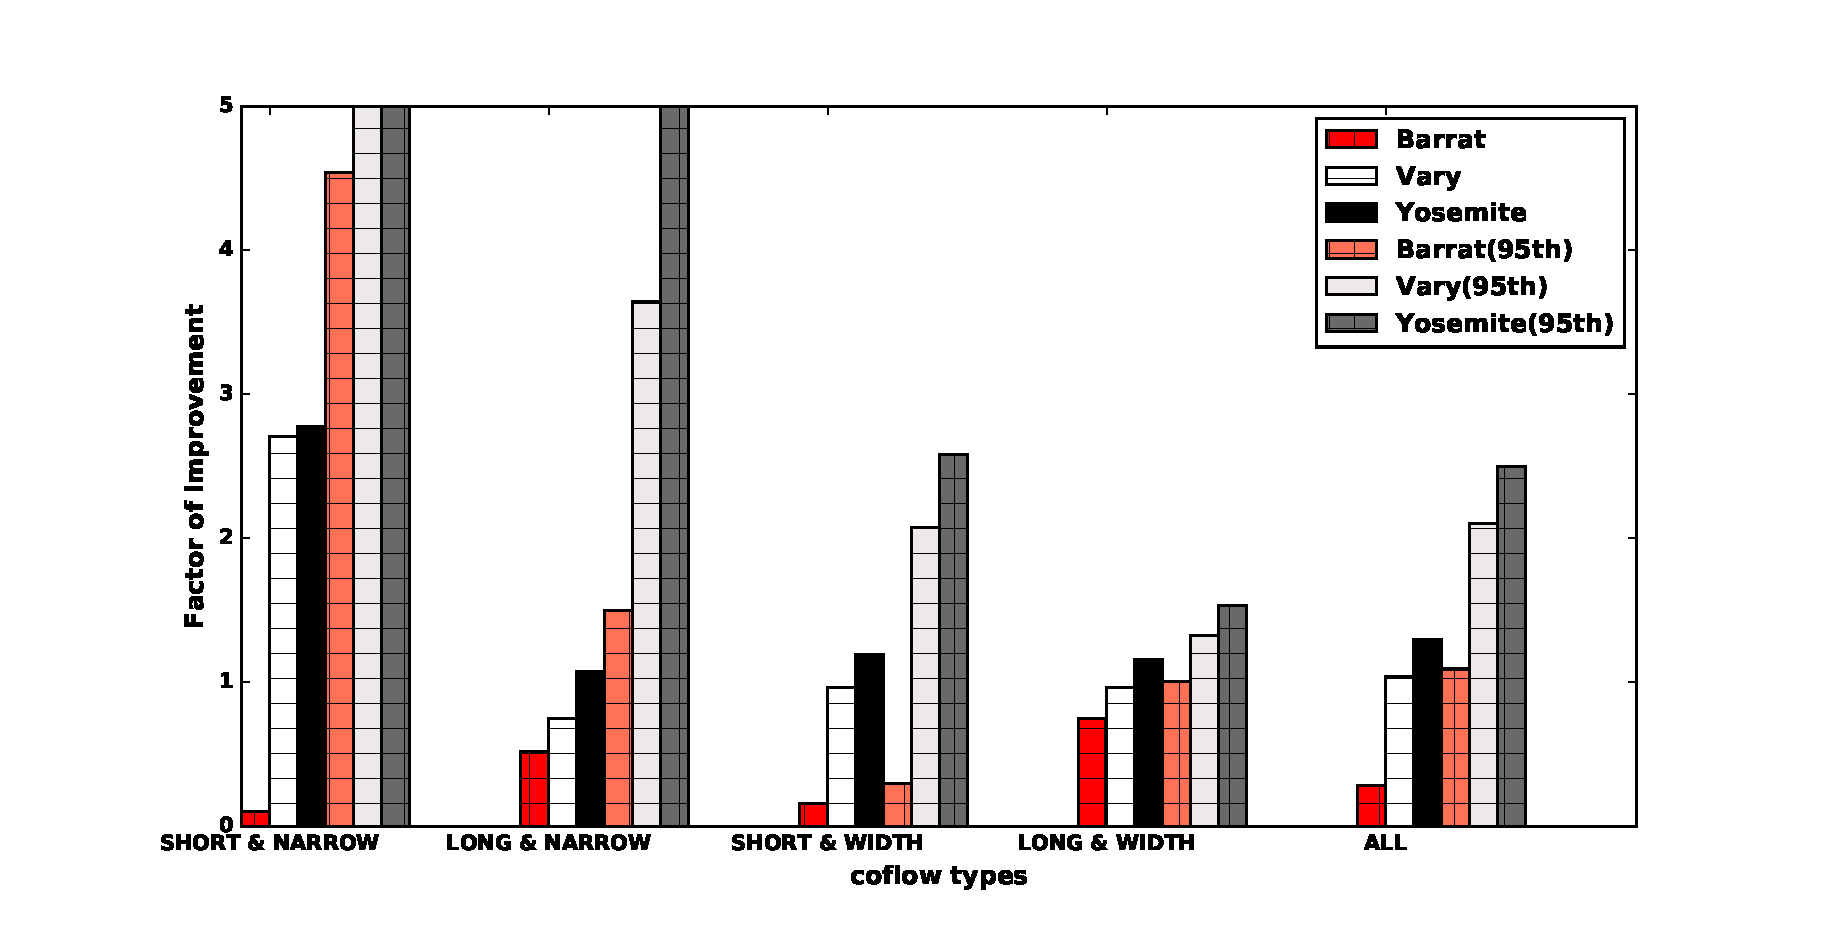
\includegraphics[width=5 in]{./figs/real/real_type.eps}}
\label{evalution_principle_b}
\hspace{0.1in}
\subfigure[Short coflow weight completion time] {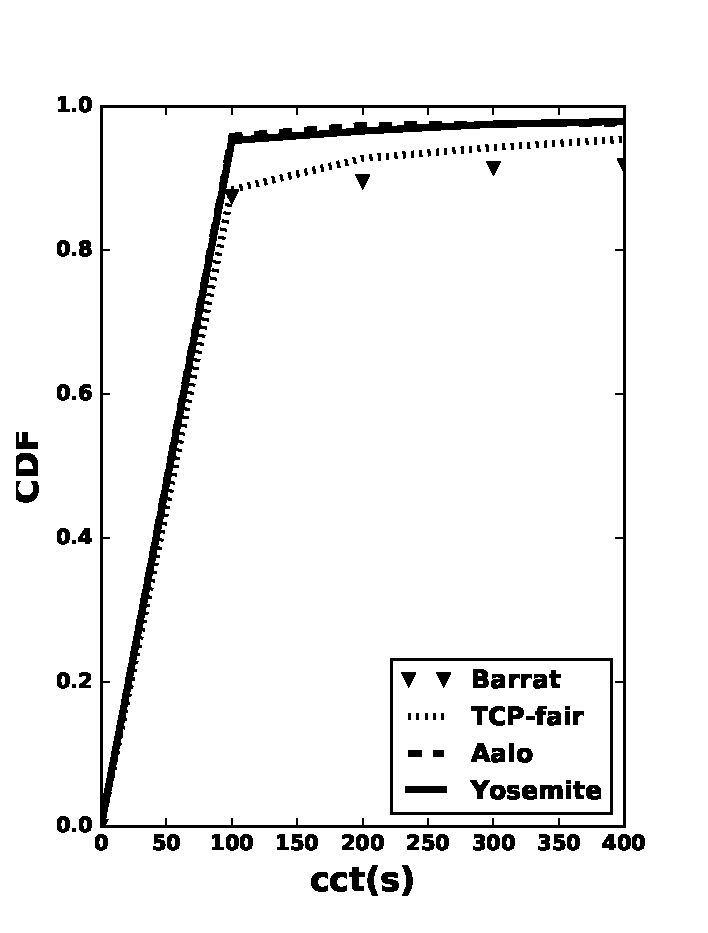
\includegraphics[width=1.9 in]{./figs/real/CDF_compare.eps}}
\vspace{-0.1 in}
\label{evalution_cases_principle_fig}
\vspace{-0.1 in}
\end{figure*}

%
%
\begin{figure*}[!t]
\centering
\subfigure[Total weight completion time] {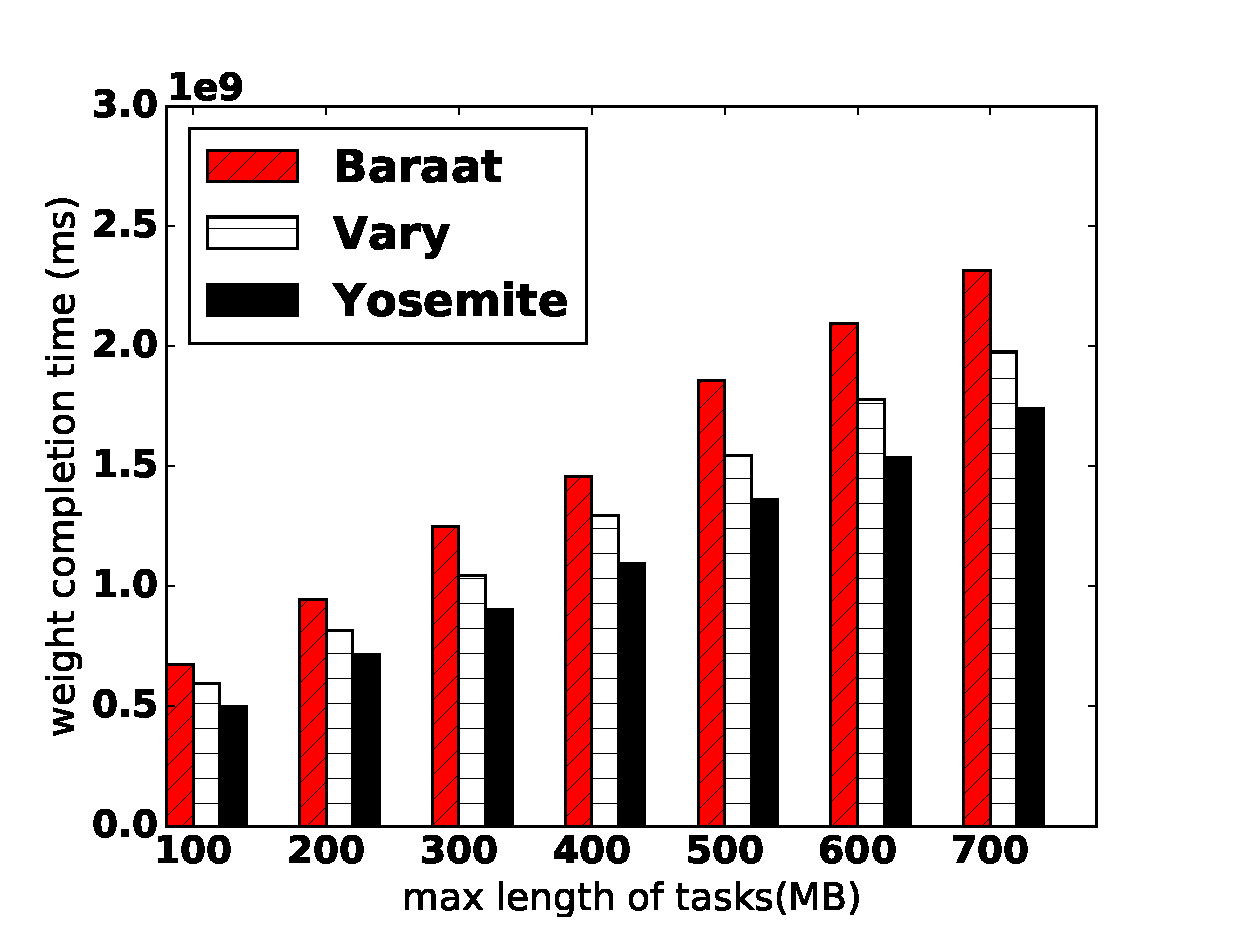
\includegraphics[width=1.65 in]{./figs/maxlength/total_completion_time.eps}}
\label{evalution_principle_b}
\hspace{0.1in}
\subfigure[Large coflow weight completion time] {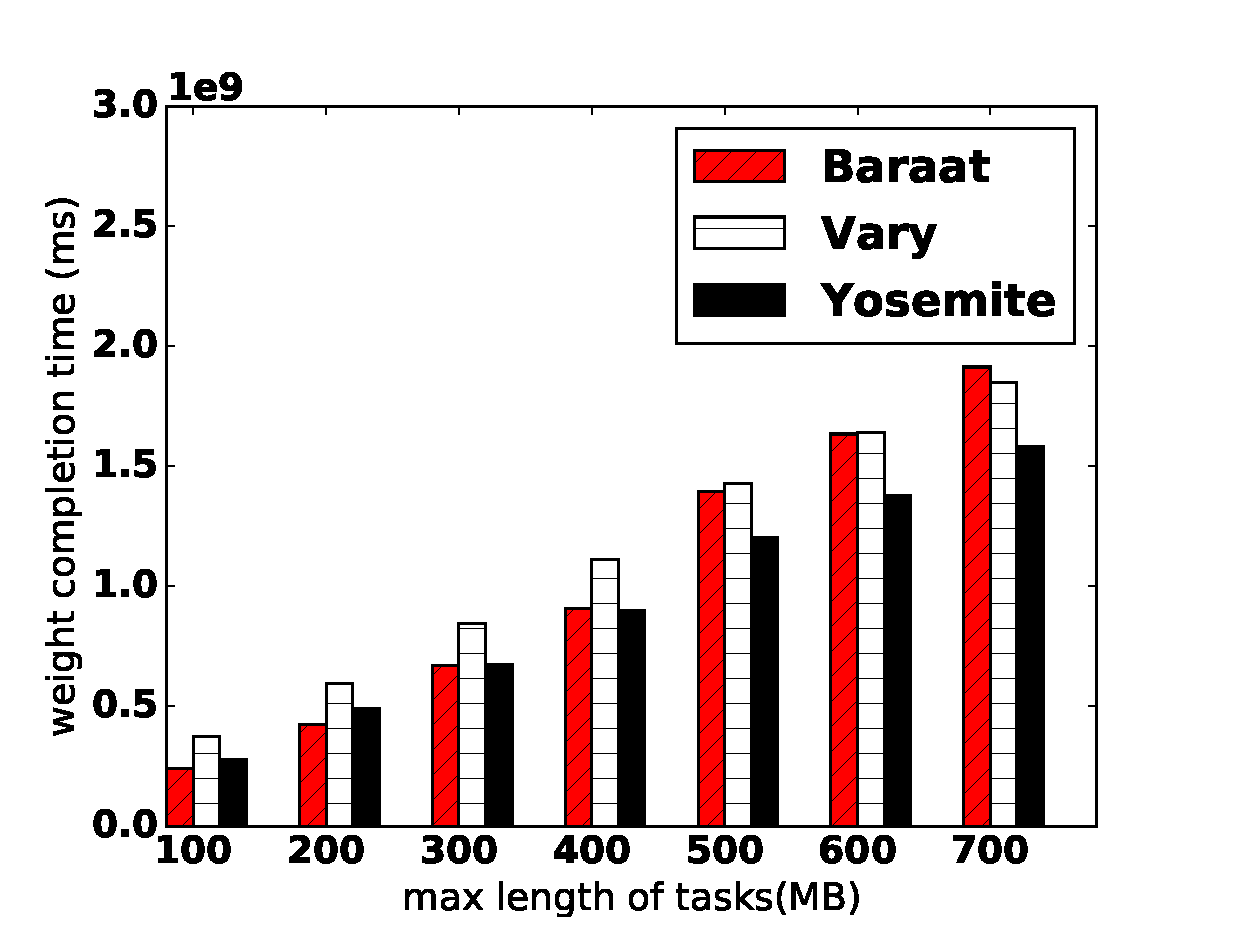
\includegraphics[width=1.65 in]{./figs/maxlength/large_completion_time.eps}}
\label{evalution_principle_w}
\hspace{0.1in}
\subfigure[Short coflow weight completion time] {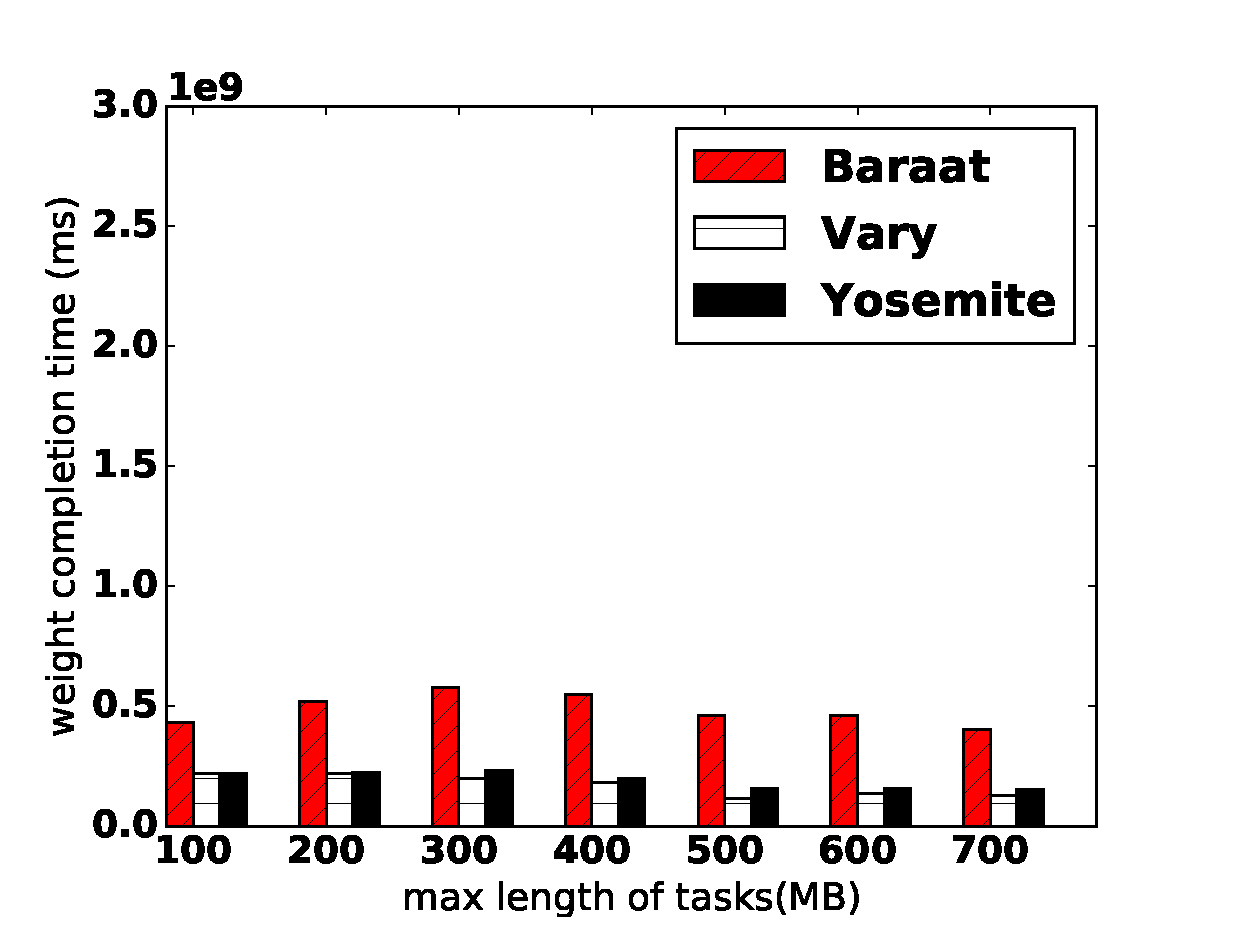
\includegraphics[width=1.65 in]{./figs/maxlength/short_completion_time.eps}}
\vspace{-0.1 in}
\subfigure[Improvement over Baraat] {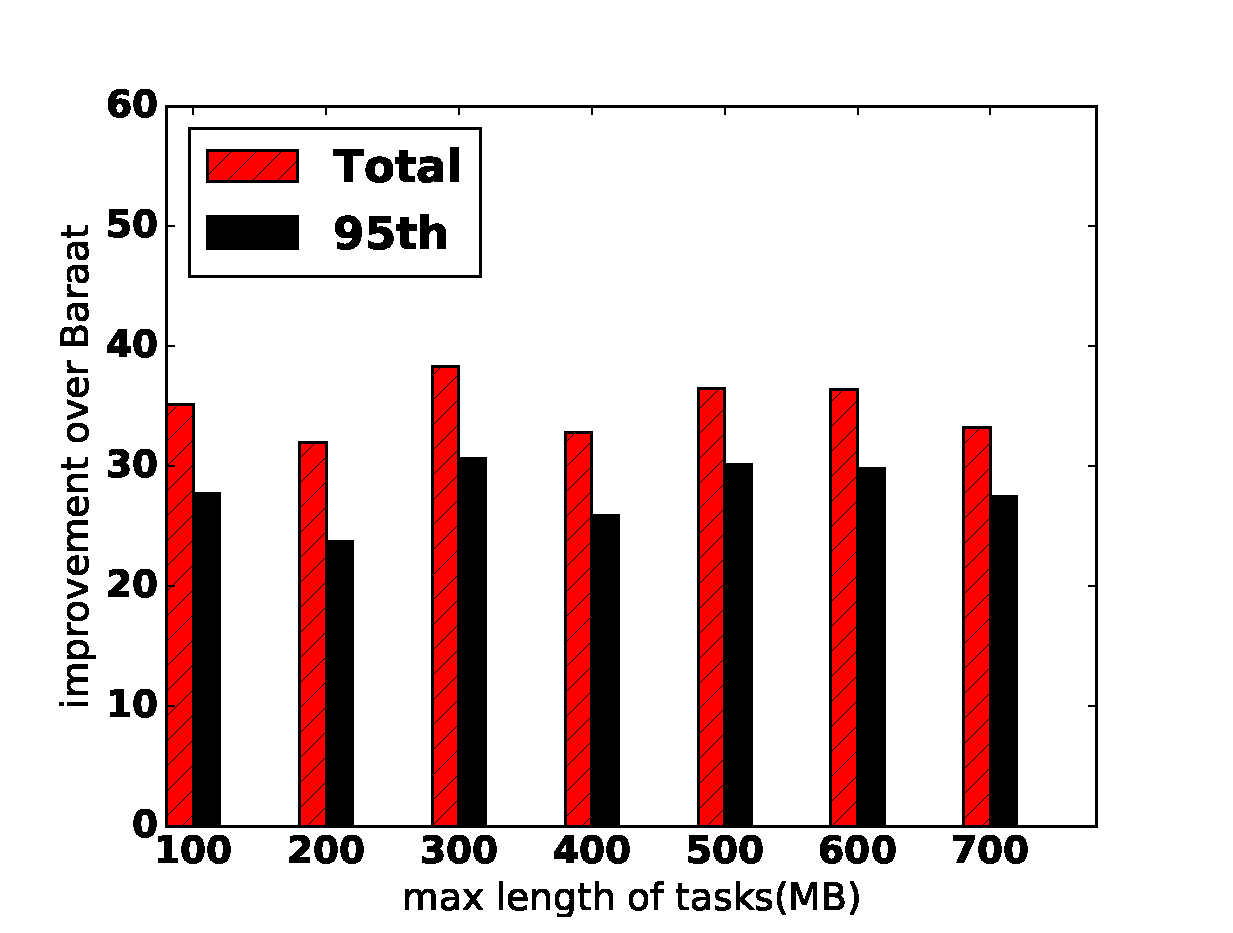
\includegraphics[width=1.65 in]{./figs/maxlength/improvement.eps}}
\caption{Yosemite performance comparison with Baraat and Varys when the max length of coflows increasing }
\label{evalution_cases_principle_fig}
\vspace{-0.1 in}
\end{figure*}
%
%
%
%
\begin{figure*}[!t]
\centering
\subfigure[Total weight completion time] {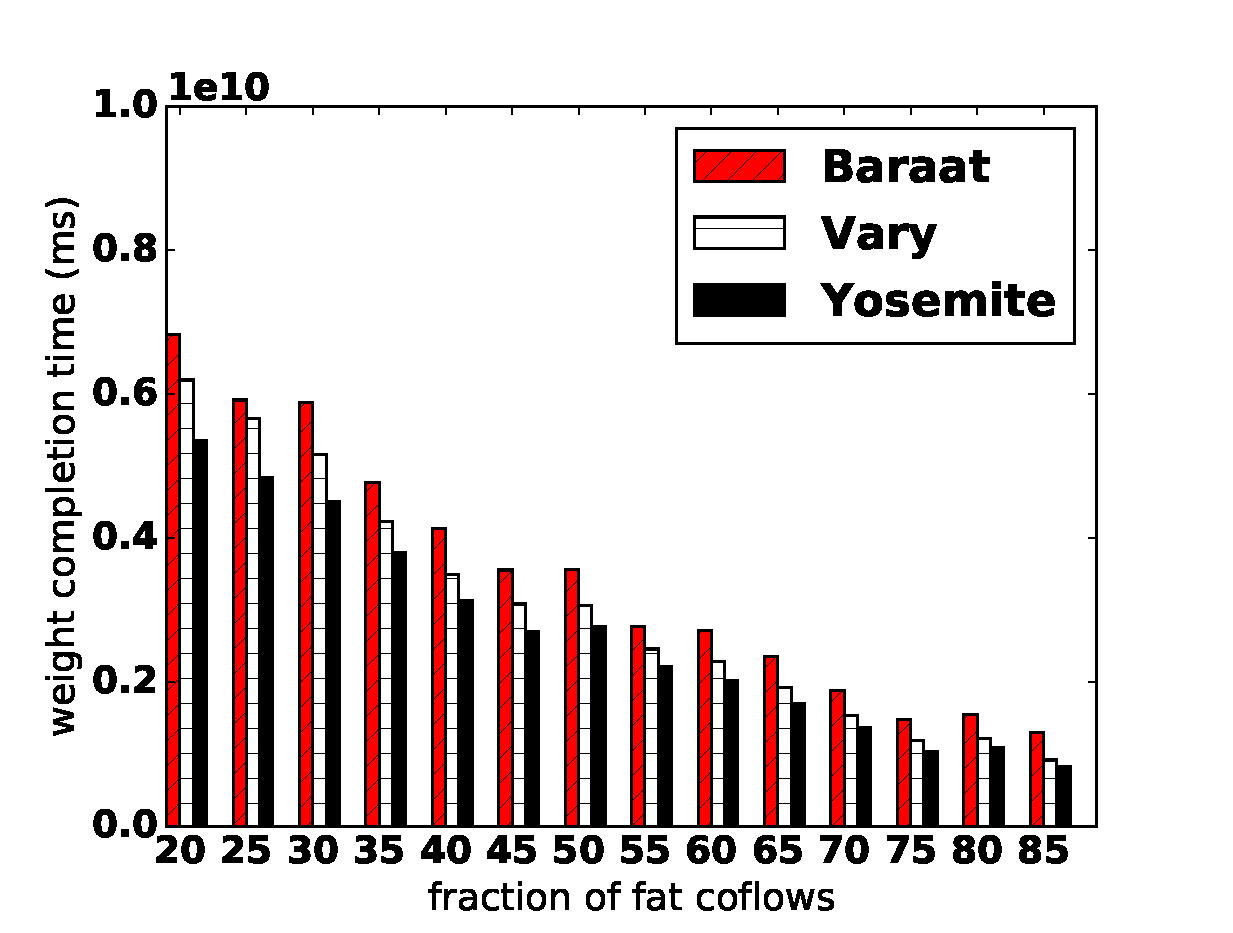
\includegraphics[width=1.65 in]{./figs/width/total_completion_time.eps}}
\label{evalution_principle_b}
\hspace{0.1in}
\subfigure[Large coflow weight completion time] {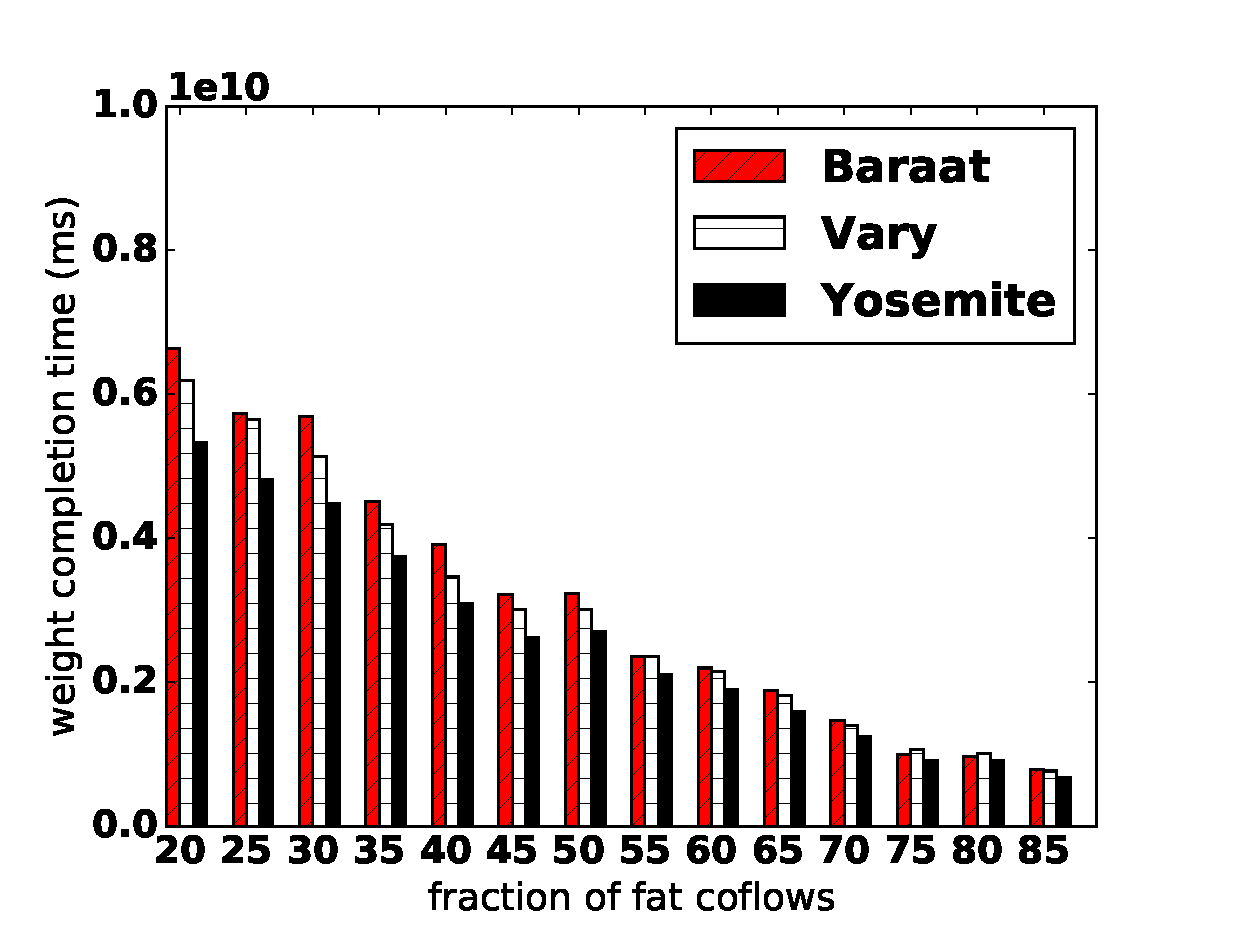
\includegraphics[width=1.65 in]{./figs/width/large_completion_time.eps}}
\label{evalution_principle_w}
\hspace{0.1in}
\subfigure[Short coflow weight completion time] {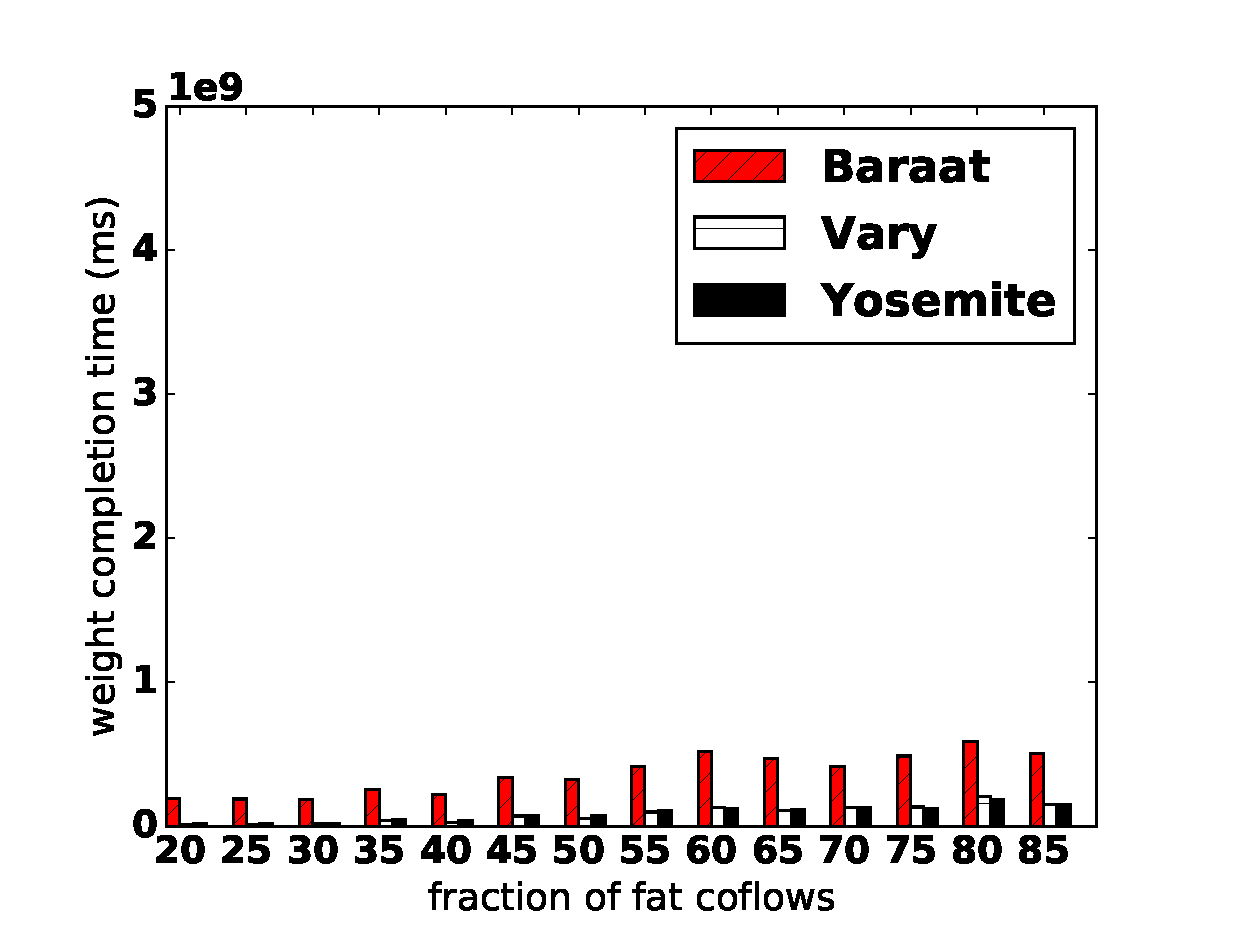
\includegraphics[width=1.65 in]{./figs/width/short_completion_time.eps}}
\vspace{-0.1 in}
\subfigure[Improvement over Baraat] {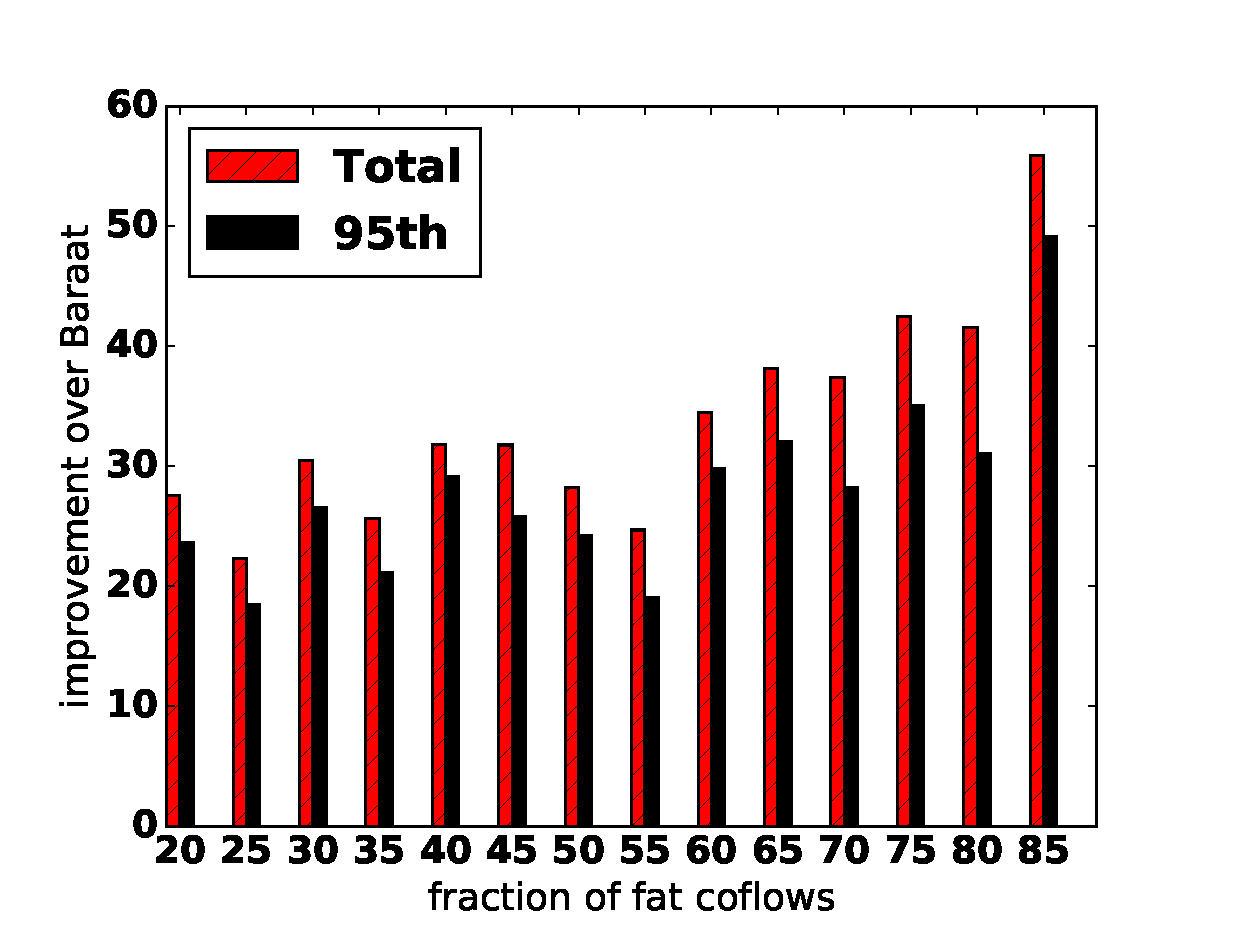
\includegraphics[width=1.65 in]{./figs/width/improvement.eps}}
\caption{Yosemite performance comparison with Baraat and Varys under different percentage of width coflows }
\label{evalution_cases_principle_fig}
\vspace{-0.1 in}
\end{figure*}


\bibliographystyle{abbrv}
\bibliography{paper}



\end{document}



